\pdfminorversion=4 % for acroread
%\documentclass[aspectratio=169,t,xcolor={usenames,dvipsnames}]{beamer}
\documentclass[aspectratio=169,t,handout,xcolor={usenames,dvipsnames}]{beamer}
\usepackage{../beamerstyle}
\usepackage{dsfont}
\usepackage{bm}
\usepackage[english]{babel}
\usepackage[utf8]{inputenc}
\usepackage{graphicx}
\usepackage{algorithm}
\usepackage[ruled,vlined,algo2e,linesnumbered]{algorithm2e}
%\usepackage[boxed,vlined]{algorithm2e}
\usepackage{hyperref}
\usepackage{booktabs}
\usepackage{mathtools}

\usepackage{amsmath,amssymb}
\usepackage{listings}
\lstset{frame=lines,framesep=3pt,numbers=left,numberblanklines=false,basicstyle=\ttfamily\small}

\usepackage{subfig}
\usepackage{multicol}
%\usepackage{appendixnumberbeamer}
%
\usepackage{tcolorbox}

\usepackage{pgfplots}
\usepackage{tikz}
\usetikzlibrary{trees} 
\usetikzlibrary{shapes.geometric}
\usetikzlibrary{positioning,shapes,shadows,arrows,calc,mindmap}
\usetikzlibrary{positioning,fadings,through}
\usetikzlibrary{decorations.pathreplacing}
\usetikzlibrary{intersections}
\usetikzlibrary{positioning,fit,calc,shadows,backgrounds}
\pgfdeclarelayer{background}
\pgfdeclarelayer{foreground}
\pgfsetlayers{background,main,foreground}
\tikzstyle{activity}=[rectangle, draw=black, rounded corners, text centered, text width=8em]
\tikzstyle{data}=[rectangle, draw=black, text centered, text width=8em]
\tikzstyle{myarrow}=[->, thick, draw=black]

% Define the layers to draw the diagram
\pgfdeclarelayer{background}
\pgfdeclarelayer{foreground}
\pgfsetlayers{background,main,foreground}

%\usepackage{listings}
%\lstset{numbers=left,
%  showstringspaces=false,
%  frame={tb},
%  captionpos=b,
%  lineskip=0pt,
%  basicstyle=\ttfamily,
%%  extendedchars=true,
%  stepnumber=1,
%  numberstyle=\small,
%  xleftmargin=1em,
%  breaklines
%}

 
\definecolor{blue}{RGB}{0, 74, 153}

\usetheme{Boadilla}
%\useinnertheme{rectangles}
\usecolortheme{whale}
\setbeamercolor{alerted text}{fg=blue}
\useoutertheme{infolines}
\setbeamertemplate{navigation symbols}{\vspace{-5pt}} % to lower the logo
\setbeamercolor{date in head/foot}{bg=white} % blue
\setbeamercolor{date in head/foot}{fg=white}
\setbeamercolor{author  in head/foot}{bg=white} %blue
\setbeamercolor{title in head/foot}{bg=white} % blue
\setbeamercolor{title}{fg=white, bg=blue}
\setbeamercolor{block title}{fg=white,bg=blue}
\setbeamercolor{block body}{bg=blue!10}
\setbeamercolor{frametitle}{fg=white, bg=blue}
\setbeamercovered{invisible}

\makeatletter
\setbeamertemplate{footline}
{
  \leavevmode%
  \hbox{%
  \begin{beamercolorbox}[wd=.333333\paperwidth,ht=2.25ex,dp=1ex,center]{author in head/foot}%
%    \usebeamerfont{author in head/foot}\insertshortauthor
  \end{beamercolorbox}%
  \begin{beamercolorbox}[wd=.333333\paperwidth,ht=2.25ex,dp=1ex,center]{title in head/foot}%
    \usebeamerfont{title in head/foot}\insertshorttitle
  \end{beamercolorbox}%
  \begin{beamercolorbox}[wd=.333333\paperwidth,ht=2.25ex,dp=1ex,right]{date in head/foot}%
    \usebeamerfont{date in head/foot}\insertshortdate{}\hspace*{2em}
%    \insertframenumber\hspace*{2ex} 
  \end{beamercolorbox}}%
  \vskip0pt%
}
\makeatother

%\pgfdeclareimage[height=1.2cm]{automl}{images/logos/automl.png}
%\pgfdeclareimage[height=1.2cm]{freiburg}{images/logos/freiburg}

%\logo{\pgfuseimage{freiburg}}

\renewcommand{\comment}[1]{
	\noindent
	%\vspace{0.25cm}
	{\color{red}{\textbf{TODO:} #1}}
	%\vspace{0.25cm}
}
\newcommand{\notefh}[1]{\textcolor{red}{\textbf{FH:} #1}}
\renewcommand{\comment}[1]{}
\newcommand{\hide}[1]{}
\newcommand{\cemph}[2]{\emph{\textcolor{#1}{#2}}}

\newcommand{\lit}[1]{{\footnotesize\color{black!60}[#1]}}

\newcommand{\litw}[1]{{\footnotesize\color{blue!20}[#1]}}


\newcommand{\myframe}[2]{\begin{frame}[c]{#1}#2\end{frame}}
\newcommand{\myframetop}[2]{\begin{frame}{#1}#2\end{frame}}
\newcommand{\myit}[1]{\begin{itemize}#1\end{itemize}}
\newcommand{\myblock}[2]{\begin{block}{#1}#2\end{block}}


\newcommand{\votepurple}[1]{\textcolor{Purple}{$\bigstar$}}
\newcommand{\voteyellow}[1]{\textcolor{Goldenrod}{$\bigstar$}}
\newcommand{\voteblue}[1]{\textcolor{RoyalBlue}{$\bigstar$}}
\newcommand{\votepink}[1]{\textcolor{Pink}{$\bigstar$}}

\newcommand{\diff}{\mathop{}\!\mathrm{d}}
\newcommand{\refstyle}[1]{{\small{\textcolor{gray}{#1}}}}
\newcommand{\hands}[0]{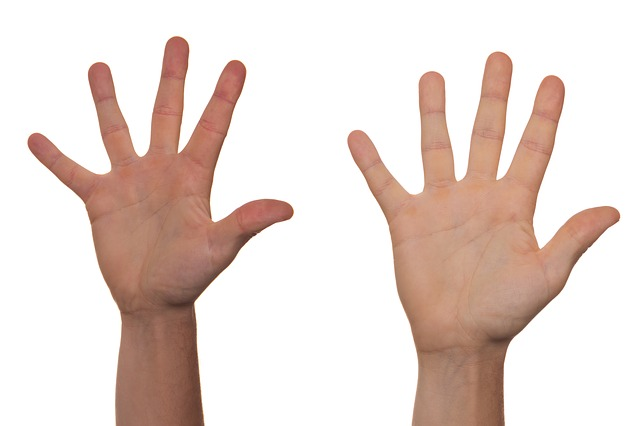
\includegraphics[height=1.5em]{images/hands}}
\newcommand{\transpose}[0]{{\textrm{\tiny{\sf{T}}}}}
\newcommand{\norm}{{\mathcal{N}}}
\newcommand{\cutoff}[0]{\kappa}
\newcommand{\instD}[0]{\dataset}
\newcommand{\insts}[0]{\mathcal{I}}
\newcommand{\inst}[0]{i}
\newcommand{\instI}[1]{i^{(#1)}}

% Iteration specific instance of variable/function/anything
% Introduced in the BO section, but moved up here to make it available within other macros
\newcommand{\iter}[2][\bocount]{{#2}^{(#1)}}

%--------HPO parameter macros-----------

% Parameter Configuration Space
\newcommand{\pcs}[0]{\pmb{\Lambda}}

% ???
\newcommand{\bx}[0]{\conf}

% Parameter Configuration
\newcommand{\conf}[0]{\pmb{\lambda}}

% Final Configuration
\newcommand{\finconf}[0]{\pmb{\hat{\lambda}}}

% Configuration corresponding to a given iteration -- better use \iter!
\newcommand{\confI}[1]{{\conf}^{(#1)}}

% Default Configuration
\newcommand{\defconf}[0]{{\conf}_{\text{def}}}

% Incumbent Configuration
\newcommand{\incumbent}[1][\bocount]{\iter[#1]{\finconf}}

% Optimal Configuration
\newcommand{\optconf}[0]{{\conf}^*}

% Configuration Space
\newcommand{\confs}[0]{\pcs}

%----------------------------------------

%\newcommand{\vlambda}[0]{\bm{\lambda}}
%\newcommand{\vLambda}[0]{\bm{\Lambda}}
\newcommand{\dataset}[0]{\mathcal{D}}
\newcommand{\datasets}[0]{\mathbf{D}}
\newcommand{\loss}[0]{L}
\newcommand{\risk}{\mathcal{R}}
\newcommand{\riske}{\mathcal{R}_{\text{emp}}}
\newcommand{\cost}[0]{c}
\newcommand{\costI}[1]{c^{(#1)}}

% Gaussian Process
\newcommand{\gp}{\mathcal{G}}
% Family of Objective Functions
\newcommand{\objF}{F}

%---------------BO Macros------------------

% BO loop counter
\newcommand{\bocount}{t}
% BO loop counter max, the counter runs from 1 to this value
\newcommand{\bobudget}{T}
% BO loop observation
\newcommand{\obs}[1][\conf]{\cost({#1})}
% BO loop observation space
\newcommand{\obsspace}{\mathcal{Y}}
% BO loop next observation
\newcommand{\bonextobs}{\obs[\iter{\conf}]}
% Acquisition Function, no args
\newcommand{\acq}{u}
% Standard Normal PDF
\newcommand{\pdf}{\phi}
% Standard Normal CDF
\newcommand{\cdf}{\Phi}
% Mean
\newcommand{\mean}{\mu}
% Standard Deviation
\newcommand{\stddev}{\sigma}
% Variance
\newcommand{\variance}{\sigma^2}
% Noise
\newcommand{\noise}{\nu}
% BO loop next selected sample
\newcommand{\bonextsample}{\confI{\bocount}}

% Single hyperparameter
\newcommand{\hyperparam}{\lambda}

% Single hyperparameter within a hyperparameter configuration
\newcommand{\hyperparami}[1][i]{{\hyperparam}_#1}

% Full definition of final configuration
\newcommand{\finconffull}{\incumbent[\bobudget]}

% Dataset
\newcommand{\datasetHPO}{{\dataset}_{HPO}}

% Dataset definition
\newcommand{\datasetHPOdef}{{\langle \bonextsample,\,\bonextobs \rangle}_{\bocount=1}^{\bobudget}}

% Double Display Fraction, forces large displays for everything in numerator and denominator
\newcommand\ddfrac[2]{\frac{\displaystyle #1}{\displaystyle #2}}

% Conditional Probability "Given That" Relation, source:https://tex.stackexchange.com/a/141685/205886
\newcommand\given[1][]{\:#1\vert\:}

% Expectation as a math operator
\DeclareMathOperator*{\E}{\mathbb{E}}

% Citation 
\newcommand{\source}[1]{
    \begin{flushright}
    	Source: \lit{#1}
    \end{flushright}
}
%-------------------------------------------

%Real numbers set
\newcommand{\realnum}{\mathbb{R}}
%Configuration space - do not use
%\newcommand{\configspace}{\Theta}
%Instances - do not use
%\newcommand{\instances}{\mathcal{I}}
%Expected value
\newcommand{\expectation}{\mathbb{E}}
%Kernel
\newcommand{\kernel}{\kappa}
%Constraint function
\newcommand{\constraintf}{c}
%Normal distribution
\newcommand{\normaldist}{\mathcal{N}}

% \renewcommand{\vec}[1]{\mathbf{#1}}
\newcommand{\hist}[0]{\dataset_{\text{Hist}}}
\newcommand{\param}[0]{p}
\newcommand{\algo}[0]{\mathcal{A}}
\newcommand{\algos}[0]{\mathbf{A}}
%\newcommand{\nn}[0]{N}
\newcommand{\feats}[0]{\mathcal{X}_{\text{meta}}}
\newcommand{\feat}[0]{\x_{\text{meta}}}
%\newcommand{\cluster}[0]{\vec{h}}
%\newcommand{\clusters}[0]{\vec{H}}
\newcommand{\perf}[0]{\mathbb{R}}
%\newcommand{\surro}[0]{\mathcal{S}}
\newcommand{\surro}[0]{\hat{\cost}}
\newcommand{\func}[0]{f}
\newcommand{\epm}[0]{\surro}
\newcommand{\portfolio}[0]{\mathbf{P}}
\newcommand{\schedule}[0]{\mathcal{S}}

% Machine Learning
\newcommand{\mdata}[0]{\dataset_{\text{meta}}}
\newcommand{\datasettrain}[0]{\dataset_{\text{train}}}
\newcommand{\datasetval}[0]{\dataset_{\text{val}}}
\newcommand{\datasettest}[0]{\dataset_{\text{test}}}
\newcommand{\x}[0]{\mathbf{x}}
\newcommand{\y}[0]{y}
\newcommand{\xI}[1]{\mathbf{x}^{(#1)}}
\newcommand{\yI}[1]{y^{(#1)}}
\newcommand{\fx}{f(\mathbf{x})}  % f(x), continuous prediction function
\newcommand{\Hspace}{\mathcal{H}} % hypothesis space where f is from
\newcommand{\fh}{\hat{f}}       % f hat, estimated prediction function

% Deep Learning
\newcommand{\weights}[0]{\theta}
\newcommand{\metaweights}[0]{\phi}


% reinforcement learning
\newcommand{\policies}[0]{\mathbf{\Pi}}
\newcommand{\policy}[0]{\pi}
\newcommand{\actionRL}[0]{a}
\newcommand{\stateRL}[0]{s}
\newcommand{\statesRL}[0]{\mathcal{S}}
\newcommand{\rewardRL}[0]{r}
\newcommand{\rewardfuncRL}[0]{\mathcal{R}}

\RestyleAlgo{algoruled}
\DontPrintSemicolon
\LinesNumbered
\SetAlgoVlined
\SetFuncSty{textsc}

\SetKwInOut{Input}{Input}
\SetKwInOut{Output}{Output}
\SetKw{Return}{return}

%\newcommand{\changed}[1]{{\color{red}#1}}

%\newcommand{\citeN}[1]{\citeauthor{#1}~(\citeyear{#1})}

\renewcommand{\vec}[1]{\mathbf{#1}}
\DeclareMathOperator*{\argmin}{arg\,min}
\DeclareMathOperator*{\argmax}{arg\,max}

%\newcommand{\aqme}{\textit{AQME}}
%\newcommand{\aslib}{\textit{ASlib}}
%\newcommand{\llama}{\textit{LLAMA}}
%\newcommand{\satzilla}{\textit{SATzilla}}
%\newcommand{\satzillaY}[1]{\textit{SATzilla'{#1}}}
%\newcommand{\snnap}{\textit{SNNAP}}
%\newcommand{\claspfolioTwo}{\textit{claspfolio~2}}
%\newcommand{\flexfolio}{\textit{FlexFolio}}
%\newcommand{\claspfolioOne}{\textit{claspfolio~1}}
%\newcommand{\isac}{\textit{ISAC}}
%\newcommand{\eisac}{\textit{EISAC}}
%\newcommand{\sss}{\textit{3S}}
%\newcommand{\sunny}{\textit{Sunny}}
%\newcommand{\ssspar}{\textit{3Spar}}
%\newcommand{\cshc}{\textit{CSHC}}
%\newcommand{\cshcpar}{\textit{CSHCpar}}
%\newcommand{\measp}{\textit{ME-ASP}}
%\newcommand{\aspeed}{\textit{aspeed}}
%\newcommand{\autofolio}{\textit{AutoFolio}}
%\newcommand{\cedalion}{\textit{Cedalion}}
\newcommand{\fanova}{\textit{fANOVA}}
\newcommand{\sbs}{\textit{SB}}
\newcommand{\oracle}{\textit{VBS}}

% like approaches
\newcommand{\claspfoliolike}[1]{\texttt{claspfolio-#1-like}}
\newcommand{\satzillalike}[1]{\texttt{SATzilla'#1-like}}
\newcommand{\isaclike}{\texttt{ISAC-like}}
\newcommand{\ssslike}{\texttt{3S-like}}
\newcommand{\measplike}{\texttt{ME-ASP-like}}

\newcommand{\irace}{\textit{I/F-race}}
\newcommand{\gga}{\textit{GGA}}
\newcommand{\smac}{\textit{SMAC}}
\newcommand{\paramils}{\textit{ParamILS}}
\newcommand{\spearmint}{\textit{Spearmint}}
\newcommand{\tpe}{\textit{TPE}}


\usepackage{pifont}
\newcommand{\itarrow}{\mbox{\Pisymbol{pzd}{229}}}
\newcommand{\ithook}{\mbox{\Pisymbol{pzd}{52}}}
\newcommand{\itcross}{\mbox{\Pisymbol{pzd}{56}}}
\newcommand{\ithand}{\mbox{\raisebox{-1pt}{\Pisymbol{pzd}{43}}}}

%\DeclareMathOperator*{\argmax}{arg\,max}

\newcommand{\ie}{{\it{}i.e.\/}}
\newcommand{\eg}{{\it{}e.g.\/}}
\newcommand{\cf}{{\it{}cf.\/}}
\newcommand{\wrt}{\mbox{w.r.t.}}
\newcommand{\vs}{{\it{}vs\/}}
\newcommand{\vsp}{{\it{}vs\/}}
\newcommand{\etc}{{\copyedit{etc.}}}
\newcommand{\etal}{{\it{}et al.\/}}

\newcommand{\pscProc}{{\bf procedure}}
\newcommand{\pscBegin}{{\bf begin}}
\newcommand{\pscEnd}{{\bf end}}
\newcommand{\pscEndIf}{{\bf endif}}
\newcommand{\pscFor}{{\bf for}}
\newcommand{\pscEach}{{\bf each}}
\newcommand{\pscThen}{{\bf then}}
\newcommand{\pscElse}{{\bf else}}
\newcommand{\pscWhile}{{\bf while}}
\newcommand{\pscIf}{{\bf if}}
\newcommand{\pscRepeat}{{\bf repeat}}
\newcommand{\pscUntil}{{\bf until}}
\newcommand{\pscWithProb}{{\bf with probability}}
\newcommand{\pscOtherwise}{{\bf otherwise}}
\newcommand{\pscDo}{{\bf do}}
\newcommand{\pscTo}{{\bf to}}
\newcommand{\pscOr}{{\bf or}}
\newcommand{\pscAnd}{{\bf and}}
\newcommand{\pscNot}{{\bf not}}
\newcommand{\pscFalse}{{\bf false}}
\newcommand{\pscEachElOf}{{\bf each element of}}
\newcommand{\pscReturn}{{\bf return}}

%\newcommand{\param}[1]{{\sl{}#1}}
\newcommand{\var}[1]{{\it{}#1}}
\newcommand{\cond}[1]{{\sf{}#1}}
%\newcommand{\state}[1]{{\sf{}#1}}
%\newcommand{\func}[1]{{\sl{}#1}}
\newcommand{\set}[1]{{\Bbb #1}}
%\newcommand{\inst}[1]{{\tt{}#1}}
\newcommand{\myurl}[1]{{\small\sf #1}}

\newcommand{\Nats}{{\Bbb N}}
\newcommand{\Reals}{{\Bbb R}}
\newcommand{\extset}[2]{\{#1 \; | \; #2\}}

\newcommand{\vbar}{$\,\;|$\hspace*{-1em}\raisebox{-0.3mm}{$\,\;\;|$}}
\newcommand{\vendbar}{\raisebox{+0.4mm}{$\,\;|$}}
\newcommand{\vend}{$\,\:\lfloor$}


\newcommand{\goleft}[2][.7]{\parbox[t]{#1\linewidth}{\strut\raggedright #2\strut}}
\newcommand{\rightimage}[2][.3]{\mbox{}\hfill\raisebox{1em-\height}[0pt][0pt]{\includegraphics[width=#1\linewidth]{#2}}\vspace*{-\baselineskip}}




\usepackage{amssymb}
\usepackage{wrapfig}
\newcommand{\argminA}{\mathop{\mathrm{argmin}}}

\title[AutoML: NAS]{AutoML: Neural Architecture Search} % week title
\subtitle{Part 1: Introduction and Black-box Approaches} % video title
\author[Marius Lindauer]{Bernd Bischl \and \underline{Frank Hutter} \and Lars Kotthoff\newline \and Marius Lindauer \and Joaquin Vanschoren}
\institute{}
\date{}

\AtBeginSection[] % Do nothing for \section*
{
  \begin{frame}{Outline}
    \bigskip
    \vfill
    \tableofcontents[currentsection]
  \end{frame}
}

\begin{document}	
\maketitle

\newcommand{\lecturetitle}{Neural Architecture Search (NAS)}
\newcommand{\lecturetime}{Week 9}


\pdfminorversion=4 % for acroread
%\documentclass[aspectratio=169,t,xcolor={usenames,dvipsnames}]{beamer}
\documentclass[aspectratio=169,t,handout,xcolor={usenames,dvipsnames}]{beamer}
\usepackage{../beamerstyle}
\usepackage{dsfont}
\usepackage{bm}
\usepackage[english]{babel}
\usepackage[utf8]{inputenc}
\usepackage{graphicx}
\usepackage{algorithm}
\usepackage[ruled,vlined,algo2e,linesnumbered]{algorithm2e}
%\usepackage[boxed,vlined]{algorithm2e}
\usepackage{hyperref}
\usepackage{booktabs}
\usepackage{mathtools}

\usepackage{amsmath,amssymb}
\usepackage{listings}
\lstset{frame=lines,framesep=3pt,numbers=left,numberblanklines=false,basicstyle=\ttfamily\small}

\usepackage{subfig}
\usepackage{multicol}
%\usepackage{appendixnumberbeamer}
%
\usepackage{tcolorbox}

\usepackage{pgfplots}
\usepackage{tikz}
\usetikzlibrary{trees} 
\usetikzlibrary{shapes.geometric}
\usetikzlibrary{positioning,shapes,shadows,arrows,calc,mindmap}
\usetikzlibrary{positioning,fadings,through}
\usetikzlibrary{decorations.pathreplacing}
\usetikzlibrary{intersections}
\usetikzlibrary{positioning,fit,calc,shadows,backgrounds}
\pgfdeclarelayer{background}
\pgfdeclarelayer{foreground}
\pgfsetlayers{background,main,foreground}
\tikzstyle{activity}=[rectangle, draw=black, rounded corners, text centered, text width=8em]
\tikzstyle{data}=[rectangle, draw=black, text centered, text width=8em]
\tikzstyle{myarrow}=[->, thick, draw=black]

% Define the layers to draw the diagram
\pgfdeclarelayer{background}
\pgfdeclarelayer{foreground}
\pgfsetlayers{background,main,foreground}

%\usepackage{listings}
%\lstset{numbers=left,
%  showstringspaces=false,
%  frame={tb},
%  captionpos=b,
%  lineskip=0pt,
%  basicstyle=\ttfamily,
%%  extendedchars=true,
%  stepnumber=1,
%  numberstyle=\small,
%  xleftmargin=1em,
%  breaklines
%}

 
\definecolor{blue}{RGB}{0, 74, 153}

\usetheme{Boadilla}
%\useinnertheme{rectangles}
\usecolortheme{whale}
\setbeamercolor{alerted text}{fg=blue}
\useoutertheme{infolines}
\setbeamertemplate{navigation symbols}{\vspace{-5pt}} % to lower the logo
\setbeamercolor{date in head/foot}{bg=white} % blue
\setbeamercolor{date in head/foot}{fg=white}
\setbeamercolor{author  in head/foot}{bg=white} %blue
\setbeamercolor{title in head/foot}{bg=white} % blue
\setbeamercolor{title}{fg=white, bg=blue}
\setbeamercolor{block title}{fg=white,bg=blue}
\setbeamercolor{block body}{bg=blue!10}
\setbeamercolor{frametitle}{fg=white, bg=blue}
\setbeamercovered{invisible}

\makeatletter
\setbeamertemplate{footline}
{
  \leavevmode%
  \hbox{%
  \begin{beamercolorbox}[wd=.333333\paperwidth,ht=2.25ex,dp=1ex,center]{author in head/foot}%
%    \usebeamerfont{author in head/foot}\insertshortauthor
  \end{beamercolorbox}%
  \begin{beamercolorbox}[wd=.333333\paperwidth,ht=2.25ex,dp=1ex,center]{title in head/foot}%
    \usebeamerfont{title in head/foot}\insertshorttitle
  \end{beamercolorbox}%
  \begin{beamercolorbox}[wd=.333333\paperwidth,ht=2.25ex,dp=1ex,right]{date in head/foot}%
    \usebeamerfont{date in head/foot}\insertshortdate{}\hspace*{2em}
%    \insertframenumber\hspace*{2ex} 
  \end{beamercolorbox}}%
  \vskip0pt%
}
\makeatother

%\pgfdeclareimage[height=1.2cm]{automl}{images/logos/automl.png}
%\pgfdeclareimage[height=1.2cm]{freiburg}{images/logos/freiburg}

%\logo{\pgfuseimage{freiburg}}

\renewcommand{\comment}[1]{
	\noindent
	%\vspace{0.25cm}
	{\color{red}{\textbf{TODO:} #1}}
	%\vspace{0.25cm}
}
\newcommand{\notefh}[1]{\textcolor{red}{\textbf{FH:} #1}}
\renewcommand{\comment}[1]{}
\newcommand{\hide}[1]{}
\newcommand{\cemph}[2]{\emph{\textcolor{#1}{#2}}}

\newcommand{\lit}[1]{{\footnotesize\color{black!60}[#1]}}

\newcommand{\litw}[1]{{\footnotesize\color{blue!20}[#1]}}


\newcommand{\myframe}[2]{\begin{frame}[c]{#1}#2\end{frame}}
\newcommand{\myframetop}[2]{\begin{frame}{#1}#2\end{frame}}
\newcommand{\myit}[1]{\begin{itemize}#1\end{itemize}}
\newcommand{\myblock}[2]{\begin{block}{#1}#2\end{block}}


\newcommand{\votepurple}[1]{\textcolor{Purple}{$\bigstar$}}
\newcommand{\voteyellow}[1]{\textcolor{Goldenrod}{$\bigstar$}}
\newcommand{\voteblue}[1]{\textcolor{RoyalBlue}{$\bigstar$}}
\newcommand{\votepink}[1]{\textcolor{Pink}{$\bigstar$}}

\newcommand{\diff}{\mathop{}\!\mathrm{d}}
\newcommand{\refstyle}[1]{{\small{\textcolor{gray}{#1}}}}
\newcommand{\hands}[0]{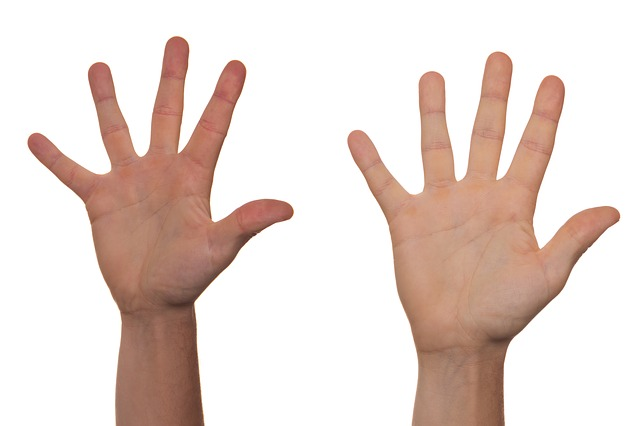
\includegraphics[height=1.5em]{images/hands}}
\newcommand{\transpose}[0]{{\textrm{\tiny{\sf{T}}}}}
\newcommand{\norm}{{\mathcal{N}}}
\newcommand{\cutoff}[0]{\kappa}
\newcommand{\instD}[0]{\dataset}
\newcommand{\insts}[0]{\mathcal{I}}
\newcommand{\inst}[0]{i}
\newcommand{\instI}[1]{i^{(#1)}}

% Iteration specific instance of variable/function/anything
% Introduced in the BO section, but moved up here to make it available within other macros
\newcommand{\iter}[2][\bocount]{{#2}^{(#1)}}

%--------HPO parameter macros-----------

% Parameter Configuration Space
\newcommand{\pcs}[0]{\pmb{\Lambda}}

% ???
\newcommand{\bx}[0]{\conf}

% Parameter Configuration
\newcommand{\conf}[0]{\pmb{\lambda}}

% Final Configuration
\newcommand{\finconf}[0]{\pmb{\hat{\lambda}}}

% Configuration corresponding to a given iteration -- better use \iter!
\newcommand{\confI}[1]{{\conf}^{(#1)}}

% Default Configuration
\newcommand{\defconf}[0]{{\conf}_{\text{def}}}

% Incumbent Configuration
\newcommand{\incumbent}[1][\bocount]{\iter[#1]{\finconf}}

% Optimal Configuration
\newcommand{\optconf}[0]{{\conf}^*}

% Configuration Space
\newcommand{\confs}[0]{\pcs}

%----------------------------------------

%\newcommand{\vlambda}[0]{\bm{\lambda}}
%\newcommand{\vLambda}[0]{\bm{\Lambda}}
\newcommand{\dataset}[0]{\mathcal{D}}
\newcommand{\datasets}[0]{\mathbf{D}}
\newcommand{\loss}[0]{L}
\newcommand{\risk}{\mathcal{R}}
\newcommand{\riske}{\mathcal{R}_{\text{emp}}}
\newcommand{\cost}[0]{c}
\newcommand{\costI}[1]{c^{(#1)}}

% Gaussian Process
\newcommand{\gp}{\mathcal{G}}
% Family of Objective Functions
\newcommand{\objF}{F}

%---------------BO Macros------------------

% BO loop counter
\newcommand{\bocount}{t}
% BO loop counter max, the counter runs from 1 to this value
\newcommand{\bobudget}{T}
% BO loop observation
\newcommand{\obs}[1][\conf]{\cost({#1})}
% BO loop observation space
\newcommand{\obsspace}{\mathcal{Y}}
% BO loop next observation
\newcommand{\bonextobs}{\obs[\iter{\conf}]}
% Acquisition Function, no args
\newcommand{\acq}{u}
% Standard Normal PDF
\newcommand{\pdf}{\phi}
% Standard Normal CDF
\newcommand{\cdf}{\Phi}
% Mean
\newcommand{\mean}{\mu}
% Standard Deviation
\newcommand{\stddev}{\sigma}
% Variance
\newcommand{\variance}{\sigma^2}
% Noise
\newcommand{\noise}{\nu}
% BO loop next selected sample
\newcommand{\bonextsample}{\confI{\bocount}}

% Single hyperparameter
\newcommand{\hyperparam}{\lambda}

% Single hyperparameter within a hyperparameter configuration
\newcommand{\hyperparami}[1][i]{{\hyperparam}_#1}

% Full definition of final configuration
\newcommand{\finconffull}{\incumbent[\bobudget]}

% Dataset
\newcommand{\datasetHPO}{{\dataset}_{HPO}}

% Dataset definition
\newcommand{\datasetHPOdef}{{\langle \bonextsample,\,\bonextobs \rangle}_{\bocount=1}^{\bobudget}}

% Double Display Fraction, forces large displays for everything in numerator and denominator
\newcommand\ddfrac[2]{\frac{\displaystyle #1}{\displaystyle #2}}

% Conditional Probability "Given That" Relation, source:https://tex.stackexchange.com/a/141685/205886
\newcommand\given[1][]{\:#1\vert\:}

% Expectation as a math operator
\DeclareMathOperator*{\E}{\mathbb{E}}

% Citation 
\newcommand{\source}[1]{
    \begin{flushright}
    	Source: \lit{#1}
    \end{flushright}
}
%-------------------------------------------

%Real numbers set
\newcommand{\realnum}{\mathbb{R}}
%Configuration space - do not use
%\newcommand{\configspace}{\Theta}
%Instances - do not use
%\newcommand{\instances}{\mathcal{I}}
%Expected value
\newcommand{\expectation}{\mathbb{E}}
%Kernel
\newcommand{\kernel}{\kappa}
%Constraint function
\newcommand{\constraintf}{c}
%Normal distribution
\newcommand{\normaldist}{\mathcal{N}}

% \renewcommand{\vec}[1]{\mathbf{#1}}
\newcommand{\hist}[0]{\dataset_{\text{Hist}}}
\newcommand{\param}[0]{p}
\newcommand{\algo}[0]{\mathcal{A}}
\newcommand{\algos}[0]{\mathbf{A}}
%\newcommand{\nn}[0]{N}
\newcommand{\feats}[0]{\mathcal{X}_{\text{meta}}}
\newcommand{\feat}[0]{\x_{\text{meta}}}
%\newcommand{\cluster}[0]{\vec{h}}
%\newcommand{\clusters}[0]{\vec{H}}
\newcommand{\perf}[0]{\mathbb{R}}
%\newcommand{\surro}[0]{\mathcal{S}}
\newcommand{\surro}[0]{\hat{\cost}}
\newcommand{\func}[0]{f}
\newcommand{\epm}[0]{\surro}
\newcommand{\portfolio}[0]{\mathbf{P}}
\newcommand{\schedule}[0]{\mathcal{S}}

% Machine Learning
\newcommand{\mdata}[0]{\dataset_{\text{meta}}}
\newcommand{\datasettrain}[0]{\dataset_{\text{train}}}
\newcommand{\datasetval}[0]{\dataset_{\text{val}}}
\newcommand{\datasettest}[0]{\dataset_{\text{test}}}
\newcommand{\x}[0]{\mathbf{x}}
\newcommand{\y}[0]{y}
\newcommand{\xI}[1]{\mathbf{x}^{(#1)}}
\newcommand{\yI}[1]{y^{(#1)}}
\newcommand{\fx}{f(\mathbf{x})}  % f(x), continuous prediction function
\newcommand{\Hspace}{\mathcal{H}} % hypothesis space where f is from
\newcommand{\fh}{\hat{f}}       % f hat, estimated prediction function

% Deep Learning
\newcommand{\weights}[0]{\theta}
\newcommand{\metaweights}[0]{\phi}


% reinforcement learning
\newcommand{\policies}[0]{\mathbf{\Pi}}
\newcommand{\policy}[0]{\pi}
\newcommand{\actionRL}[0]{a}
\newcommand{\stateRL}[0]{s}
\newcommand{\statesRL}[0]{\mathcal{S}}
\newcommand{\rewardRL}[0]{r}
\newcommand{\rewardfuncRL}[0]{\mathcal{R}}

\RestyleAlgo{algoruled}
\DontPrintSemicolon
\LinesNumbered
\SetAlgoVlined
\SetFuncSty{textsc}

\SetKwInOut{Input}{Input}
\SetKwInOut{Output}{Output}
\SetKw{Return}{return}

%\newcommand{\changed}[1]{{\color{red}#1}}

%\newcommand{\citeN}[1]{\citeauthor{#1}~(\citeyear{#1})}

\renewcommand{\vec}[1]{\mathbf{#1}}
\DeclareMathOperator*{\argmin}{arg\,min}
\DeclareMathOperator*{\argmax}{arg\,max}

%\newcommand{\aqme}{\textit{AQME}}
%\newcommand{\aslib}{\textit{ASlib}}
%\newcommand{\llama}{\textit{LLAMA}}
%\newcommand{\satzilla}{\textit{SATzilla}}
%\newcommand{\satzillaY}[1]{\textit{SATzilla'{#1}}}
%\newcommand{\snnap}{\textit{SNNAP}}
%\newcommand{\claspfolioTwo}{\textit{claspfolio~2}}
%\newcommand{\flexfolio}{\textit{FlexFolio}}
%\newcommand{\claspfolioOne}{\textit{claspfolio~1}}
%\newcommand{\isac}{\textit{ISAC}}
%\newcommand{\eisac}{\textit{EISAC}}
%\newcommand{\sss}{\textit{3S}}
%\newcommand{\sunny}{\textit{Sunny}}
%\newcommand{\ssspar}{\textit{3Spar}}
%\newcommand{\cshc}{\textit{CSHC}}
%\newcommand{\cshcpar}{\textit{CSHCpar}}
%\newcommand{\measp}{\textit{ME-ASP}}
%\newcommand{\aspeed}{\textit{aspeed}}
%\newcommand{\autofolio}{\textit{AutoFolio}}
%\newcommand{\cedalion}{\textit{Cedalion}}
\newcommand{\fanova}{\textit{fANOVA}}
\newcommand{\sbs}{\textit{SB}}
\newcommand{\oracle}{\textit{VBS}}

% like approaches
\newcommand{\claspfoliolike}[1]{\texttt{claspfolio-#1-like}}
\newcommand{\satzillalike}[1]{\texttt{SATzilla'#1-like}}
\newcommand{\isaclike}{\texttt{ISAC-like}}
\newcommand{\ssslike}{\texttt{3S-like}}
\newcommand{\measplike}{\texttt{ME-ASP-like}}

\newcommand{\irace}{\textit{I/F-race}}
\newcommand{\gga}{\textit{GGA}}
\newcommand{\smac}{\textit{SMAC}}
\newcommand{\paramils}{\textit{ParamILS}}
\newcommand{\spearmint}{\textit{Spearmint}}
\newcommand{\tpe}{\textit{TPE}}


\usepackage{pifont}
\newcommand{\itarrow}{\mbox{\Pisymbol{pzd}{229}}}
\newcommand{\ithook}{\mbox{\Pisymbol{pzd}{52}}}
\newcommand{\itcross}{\mbox{\Pisymbol{pzd}{56}}}
\newcommand{\ithand}{\mbox{\raisebox{-1pt}{\Pisymbol{pzd}{43}}}}

%\DeclareMathOperator*{\argmax}{arg\,max}

\newcommand{\ie}{{\it{}i.e.\/}}
\newcommand{\eg}{{\it{}e.g.\/}}
\newcommand{\cf}{{\it{}cf.\/}}
\newcommand{\wrt}{\mbox{w.r.t.}}
\newcommand{\vs}{{\it{}vs\/}}
\newcommand{\vsp}{{\it{}vs\/}}
\newcommand{\etc}{{\copyedit{etc.}}}
\newcommand{\etal}{{\it{}et al.\/}}

\newcommand{\pscProc}{{\bf procedure}}
\newcommand{\pscBegin}{{\bf begin}}
\newcommand{\pscEnd}{{\bf end}}
\newcommand{\pscEndIf}{{\bf endif}}
\newcommand{\pscFor}{{\bf for}}
\newcommand{\pscEach}{{\bf each}}
\newcommand{\pscThen}{{\bf then}}
\newcommand{\pscElse}{{\bf else}}
\newcommand{\pscWhile}{{\bf while}}
\newcommand{\pscIf}{{\bf if}}
\newcommand{\pscRepeat}{{\bf repeat}}
\newcommand{\pscUntil}{{\bf until}}
\newcommand{\pscWithProb}{{\bf with probability}}
\newcommand{\pscOtherwise}{{\bf otherwise}}
\newcommand{\pscDo}{{\bf do}}
\newcommand{\pscTo}{{\bf to}}
\newcommand{\pscOr}{{\bf or}}
\newcommand{\pscAnd}{{\bf and}}
\newcommand{\pscNot}{{\bf not}}
\newcommand{\pscFalse}{{\bf false}}
\newcommand{\pscEachElOf}{{\bf each element of}}
\newcommand{\pscReturn}{{\bf return}}

%\newcommand{\param}[1]{{\sl{}#1}}
\newcommand{\var}[1]{{\it{}#1}}
\newcommand{\cond}[1]{{\sf{}#1}}
%\newcommand{\state}[1]{{\sf{}#1}}
%\newcommand{\func}[1]{{\sl{}#1}}
\newcommand{\set}[1]{{\Bbb #1}}
%\newcommand{\inst}[1]{{\tt{}#1}}
\newcommand{\myurl}[1]{{\small\sf #1}}

\newcommand{\Nats}{{\Bbb N}}
\newcommand{\Reals}{{\Bbb R}}
\newcommand{\extset}[2]{\{#1 \; | \; #2\}}

\newcommand{\vbar}{$\,\;|$\hspace*{-1em}\raisebox{-0.3mm}{$\,\;\;|$}}
\newcommand{\vendbar}{\raisebox{+0.4mm}{$\,\;|$}}
\newcommand{\vend}{$\,\:\lfloor$}


\newcommand{\goleft}[2][.7]{\parbox[t]{#1\linewidth}{\strut\raggedright #2\strut}}
\newcommand{\rightimage}[2][.3]{\mbox{}\hfill\raisebox{1em-\height}[0pt][0pt]{\includegraphics[width=#1\linewidth]{#2}}\vspace*{-\baselineskip}}







\title[AutoML: Big Picture]{AutoML: Introduction}
\subtitle{The Big Picture}
\author[Marius Lindauer]{Bernd Bischl \and Frank Hutter \and Lars Kotthoff\newline \and \underline{Marius Lindauer} \and Joaquin Vanschoren}
\institute{}
\date{}



% \AtBeginSection[] % Do nothing for \section*
% {
%   \begin{frame}{Outline}
%     \bigskip
%     \vfill
%     \tableofcontents[currentsection]
%   \end{frame}
% }

\begin{document}
	
	\maketitle
	

%----------------------------------------------------------------------
%----------------------------------------------------------------------
%\begin{frame}[c]{In a Nutshell}

%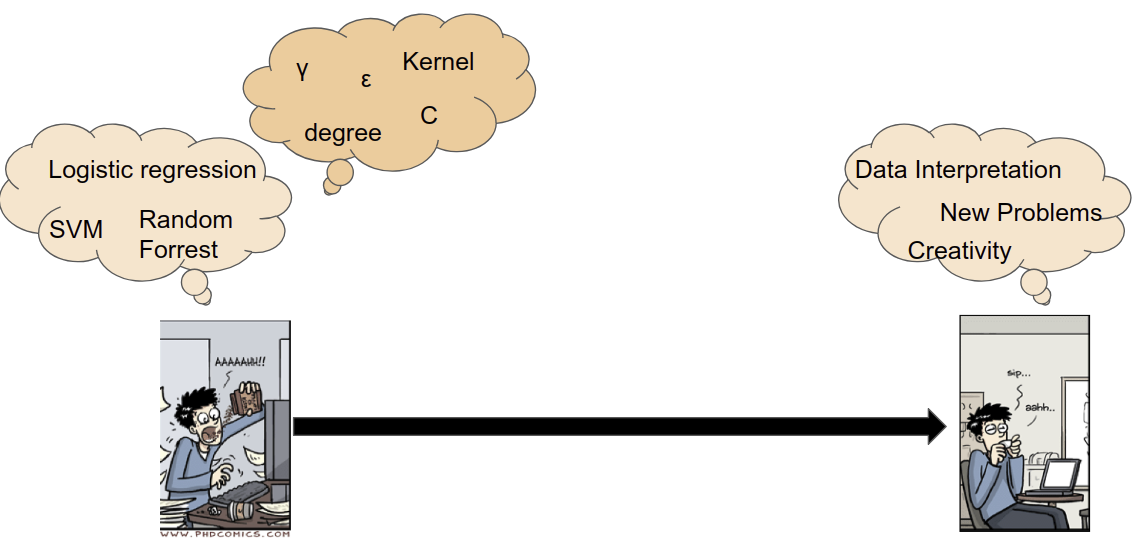
\includegraphics[width=0.99\textwidth]{images/automl_comic}

%\end{frame}
%----------------------------------------------------------------------
%----------------------------------------------------------------------
\begin{frame}[c]{Machine Learning}

\centering
\textit{``Machine learning is the science of getting computers to act\\
 without being explicitly programmed.''}

\hfill by Andrew Ng

\end{frame}
%-----------------------------------------------------------------------
%----------------------------------------------------------------------
\begin{frame}[c]{Machine Learning requires many design decisions}

\centering
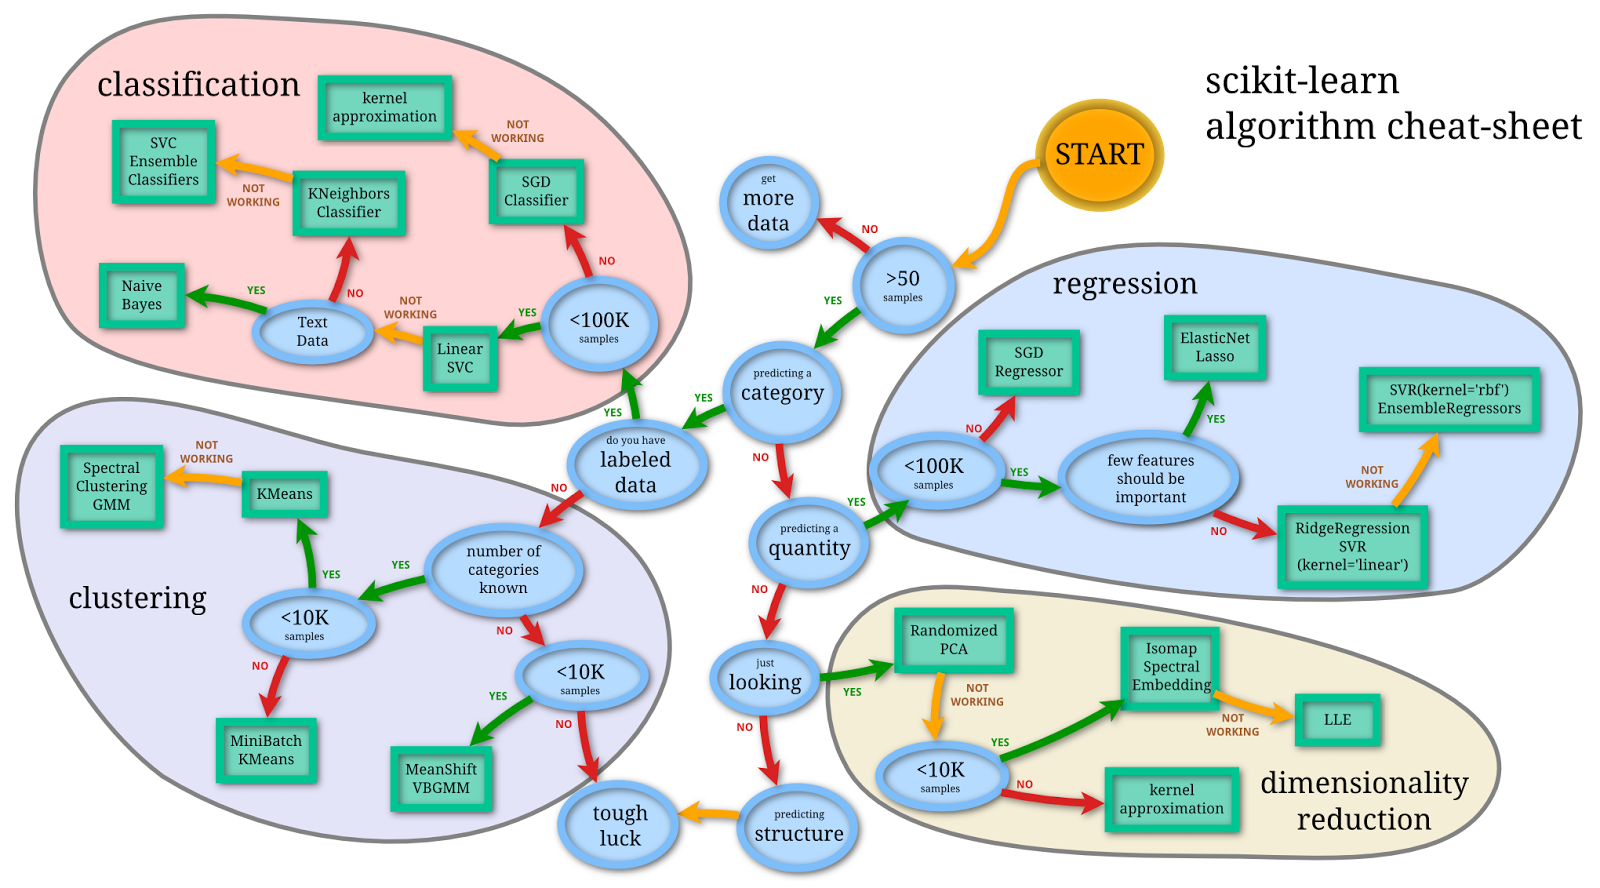
\includegraphics[width=0.8\textwidth]{images/sklearn-cheat}

\end{frame}
%-----------------------------------------------------------------------
%----------------------------------------------------------------------
\begin{frame}[c]{Machine Learning Workflow}

\centering
\tikzstyle{activity}=[rectangle, draw=black, rounded corners, text centered, text width=8em, fill=white, drop shadow]
\tikzstyle{wideactivity}=[rectangle, draw=black, rounded corners, text centered, text width=10em, fill=white, drop shadow]
\tikzstyle{data}=[rectangle, draw=black, text centered, fill=black!10, text width=8em, drop shadow]
\tikzstyle{myarrow}=[->, thick]
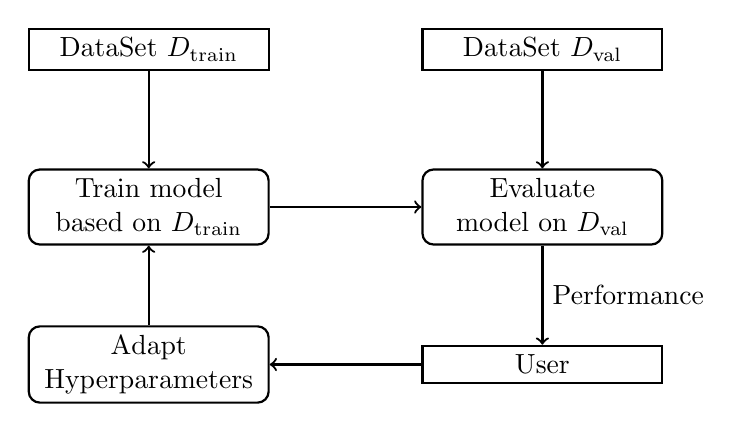
\begin{tikzpicture}[node distance=5cm,thick]
	\node (Train) [data] {DataSet $D_{\text{train}}$};
	\node (Fit) [activity, below of=Train, node distance=2cm] {Train model based on $D_{\text{train}}$};
	\draw[myarrow] (Train) -- (Fit);
	
	\pause
	
	\node (Test) [data, right of=Train] {DataSet $D_{\text{val}}$};
	\node (Eva) [activity, below of=Test, node distance=2cm] {Evaluate model on $D_{\text{val}}$};
	\draw[myarrow] (Fit) -- (Eva);
	\draw[myarrow] (Test) -- (Eva);
	
	\pause
	
	\node (user) [data, below of=Eva, node distance=2cm] {User};
	\draw[myarrow] (Eva) to node[right] {Performance} (user);
	
	\pause
	
	\node (Hyper) [activity, left of=user] {Adapt\\ Hyperparameters};
	\draw[myarrow] (user) to (Hyper);
	\draw[myarrow] (Hyper) to (Fit);
	
\end{tikzpicture}


\pause
 
\bigskip
\bigskip
\only<5->{$\leadsto$ Users indirectly teach machines how to learn.}

\end{frame}
%-----------------------------------------------------------------------
%----------------------------------------------------------------------
\begin{frame}[c]{Machine Learning does not scale up}

\begin{itemize}
  \item Basics in machine learning are not hard to grasp
  \smallskip
  \pause
  \item Achieving state-of-the-art performance is quite hard
  \smallskip
  \pause
  \item Design decisions are often not intuitive and\\ require a lot of expertise
  \begin{itemize}
    \item making these design decisions is a tedious and error-prone task
  \end{itemize}
 % \pause
  %\smallskip
%  \item Many experts are employed in ML these days
  \smallskip
  \pause
  \smallskip
  \item The job market for ML-experts is nearly empty
  \smallskip
  \pause
  \item Even with experts, developing new ML-applications takes time
\end{itemize}

\pause
\bigskip

Zoubin Ghahramani said that he often heard that:\\
\hfill \textit{``I'd like to use machine learning, but I can't invest much time.''}



\end{frame}
%-----------------------------------------------------------------------
%----------------------------------------------------------------------
%\begin{frame}[c]{AutoML Tools Demo}

%Auto-Sklearn:

%\url{https://colab.research.google.com/drive/11UcQQ_dymL5spF8o56qgSRZpMC1GKag9}

%\bigskip
%Auto-PyTorch:

%\url{https://colab.research.google.com/drive/14G5wvbqBkJ-SQJOdJsE_G8swq0JaFk6_}


%\end{frame}
%-----------------------------------------------------------------------
%----------------------------------------------------------------------
\begin{frame}[c]{Why does ML development take a lot of time?}

\centering
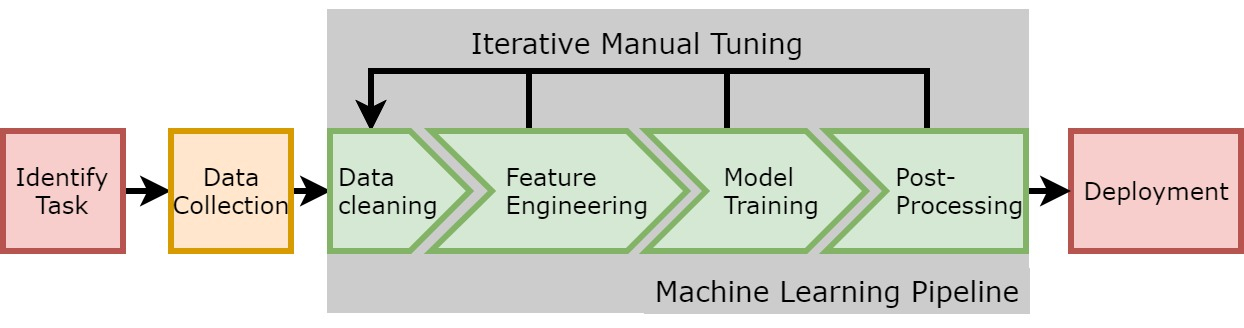
\includegraphics[width=1.0\textwidth]{images/MLPipeline.jpg}

\bigskip\bigskip\bigskip\bigskip
$\leadsto$ To achieve state-of-the-art performance,\\ this manual tuning has to be done for each new dataset again.

\end{frame}
%-----------------------------------------------------------------------
%----------------------------------------------------------------------
\begin{frame}[c]{A Simple Example with $k$-NN}

\centering
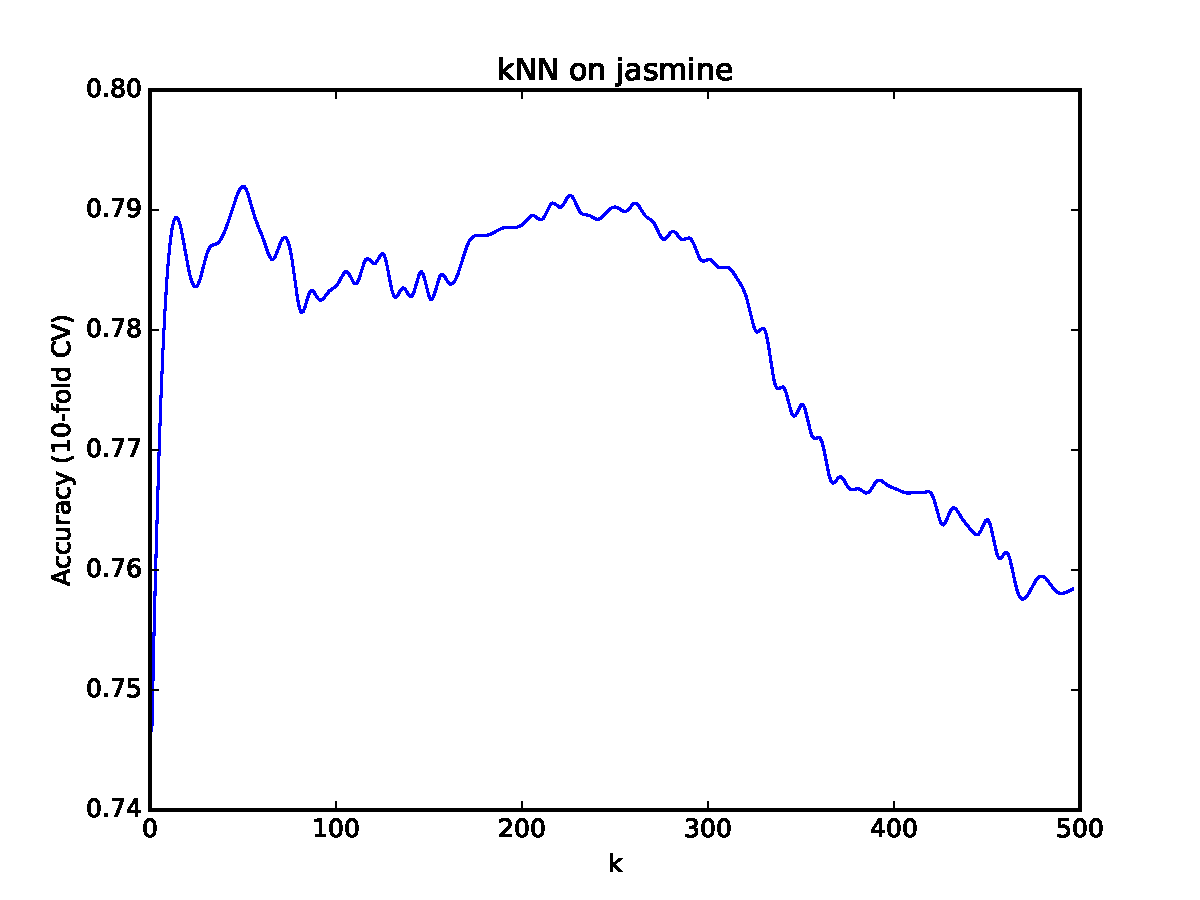
\includegraphics[width=0.5\textwidth]{images/kNN-jasmine}

\begin{itemize}
  \item $k$-nearest neighbors is one of the simplest ML algorithms
  \pause
  \item Size of neighbourhood ($k$) is very important for its performance
  \pause
  \item The performance function depending on $k$ is quite complex (not at all convex)
\end{itemize}

\end{frame}
%-----------------------------------------------------------------------
%----------------------------------------------------------------------
\begin{frame}[c]{Goal of AutoML}

\begin{block}{AutoML}
The goal of AutoML is to automate all parts of machine learning\\ (as needed)
to \emph{support} users efficiently building their ML-applications.
\end{block}

\bigskip
\pause

\begin{block}{Informal Definition: AutoML System}
Given
\begin{itemize}
  \item a dataset
  \item a task (e.g., regression or classification)
  \item a cost metric (e.g., accuracy or RMSE)
\end{itemize}
an AutoML system automatically determines the approach 
that performs best for this particular application.
\end{block}

\end{frame}
%-----------------------------------------------------------------------
%----------------------------------------------------------------------
\begin{frame}[c]{ML vs AutoML}

\begin{center}
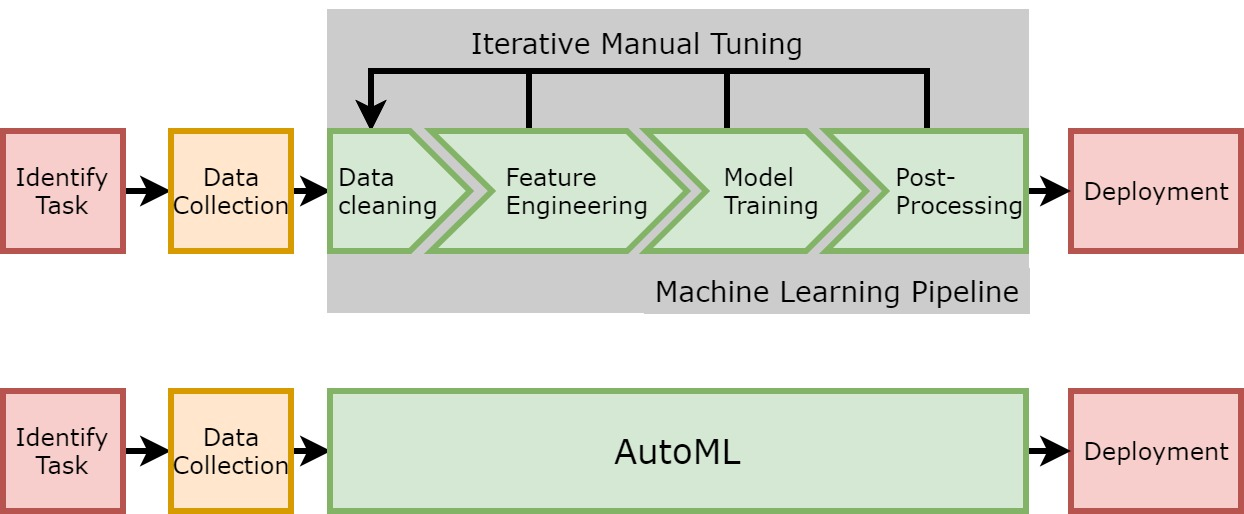
\includegraphics[width=0.7\textwidth]{images/AutoMLPipeline.jpg}
\end{center}

\bigskip
\pause
With AutoML, we ...
\begin{itemize}
	\item support ML users
	\item improve the efficiency of developping new ML applications
	\item reduce the required ML-expertise 
	\item might achieve better performance than developers w/o AutoML
\end{itemize}

\end{frame}
%-----------------------------------------------------------------------
%----------------------------------------------------------------------
\begin{frame}[c]{AutoML in Research}

AutoML enables:

\begin{enumerate}
  \item more efficient research
  \begin{itemize}
    \item AutoML has shown on subproblems to outperform human experts
  \end{itemize}
  \pause
  \smallskip
  \item more systematic research
  \begin{itemize}
    \item humans tend to be unsystematic which leads to errors
  \end{itemize}
  \smallskip
  \pause
  \item more reproducible research
  \begin{itemize}
    \item human's unsystematic approaches cannot be reproduced,\\ but AutoML is systematic
  \end{itemize}
  \smallskip
  \pause
  \item broader use of ML also in other disciplines
  \begin{itemize}
    \item ML should not be limited to computer scientists;
    \item the most amazing applications of ML are often done\\ by either interdisciplinary teams or even non-computer scientists
  \end{itemize}
\end{enumerate}

\end{frame}
%-----------------------------------------------------------------------
%----------------------------------------------------------------------
\begin{frame}[c]{Challenges in AutoML}

\begin{enumerate}
  \item Each dataset potentially require \alert{different optimal ML-designs}
  \begin{itemize}
    \item Design decisions have to be made for each dataset again
  \end{itemize}
  \smallskip
  \pause
  \item Training of a single ML model can be quite \alert{expensive}\\
  		(e.g., hours, days or weeks)
  \begin{itemize}
    \item often, we cannot try many design decisions
  \end{itemize}
  \smallskip
  \pause
  \item the \alert{mathematical relation} between design decisions\\ and performance is (often) \alert{unknown}
  \begin{itemize}
    \item gradient-based optimization is not directly possible
  \end{itemize}
  \smallskip
  \pause
  \item optimization in \alert{highly complex spaces}
  \begin{itemize}
    \item incl. categorical choices, continuous parameters,\\ conditional dependencies
  \end{itemize}
  
\end{enumerate}

\end{frame}
%-----------------------------------------------------------------------
%----------------------------------------------------------------------
%\begin{frame}[c]{Snippet of Auto-AI Hierarchy}

%\centering
%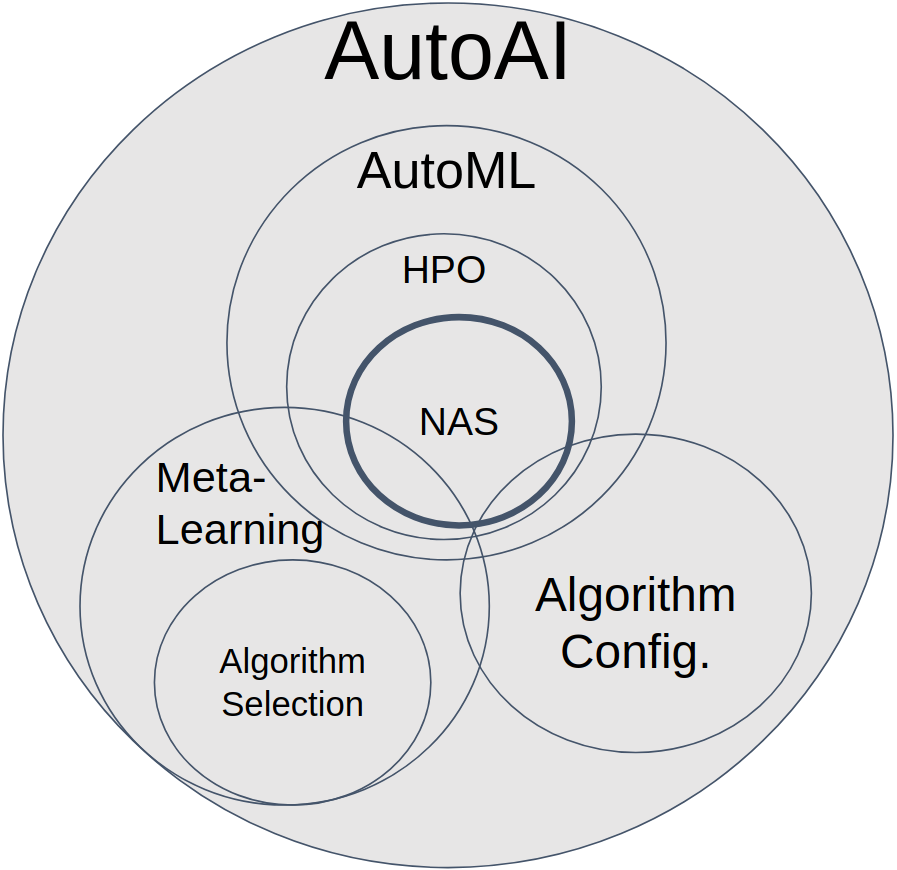
\includegraphics[width=0.5\textwidth]{images/autoai}

%\end{frame}
%-----------------------------------------------------------------------
\end{document}

\videotitle{Search Spaces}

%-------------------------------------------------
%-------------------------------------------------

%-----------------------------------------------------------------------
\myframe{Basic Neural Architecture Search Spaces}{
\centering
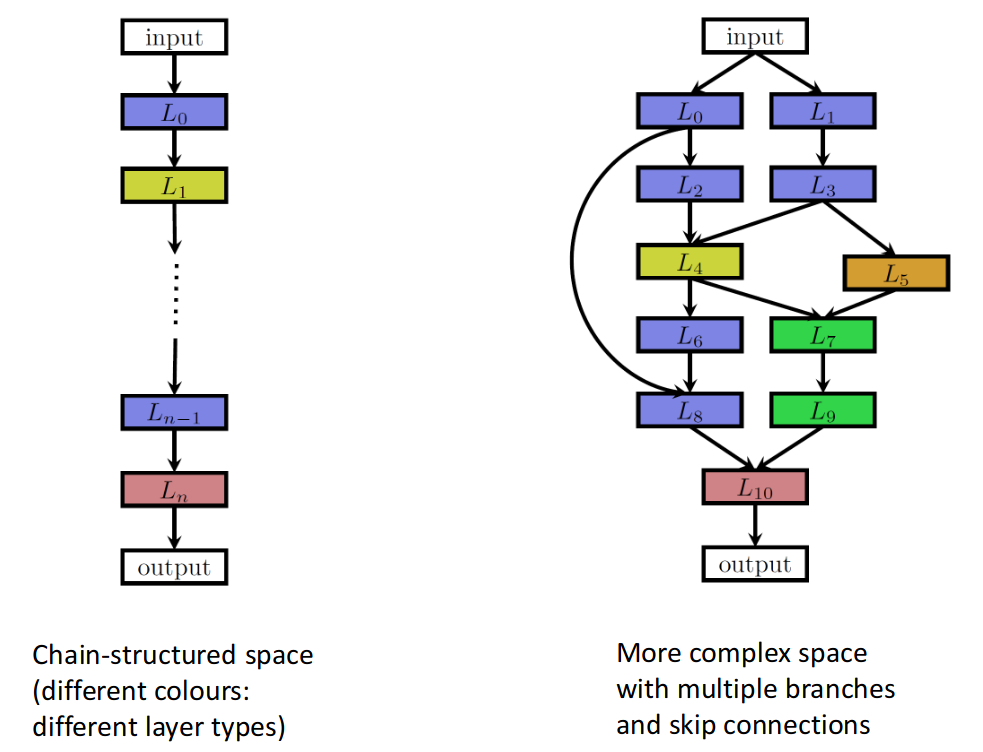
\includegraphics[height=0.9\textheight]{images/macro_space.png}
}
%----------------------------------------------------------------------

%----------------------------------------------------------------------
\myframe{Cell Search Spaces \litw{\href{https://openaccess.thecvf.com/content_cvpr_2018/papers/Zoph_Learning_Transferable_Architectures_CVPR_2018_paper.pdf}{Zoph et al. 2018}}}{
\centering
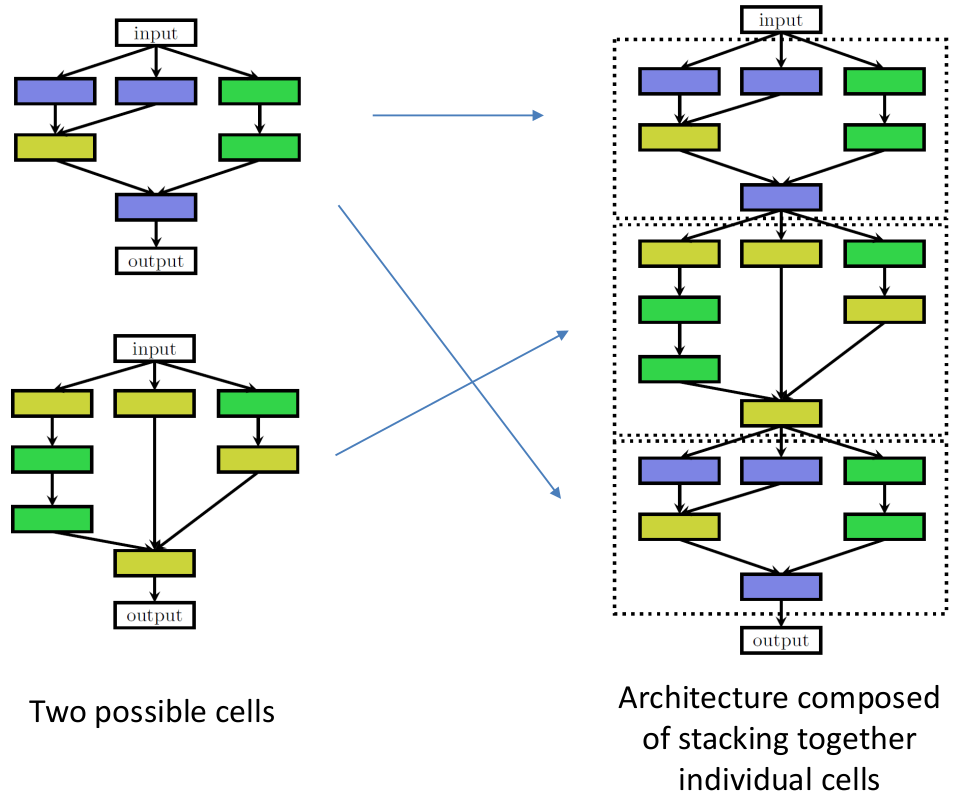
\includegraphics[height=.8\textheight]{images/s26}
}
%----------------------------------------------------------------------

%----------------------------------------------------------------------

\myframetop{Details on Cell Search Spaces \litw{\href{https://openaccess.thecvf.com/content_cvpr_2018/papers/Zoph_Learning_Transferable_Architectures_CVPR_2018_paper.pdf}{Zoph et al. 2018}}}{
	\centering
	
	\begin{itemize}
		\item 2 types of cells: normal and reduction cells
		\item For each type of cell: $B$ blocks, each with 5 choices
		\myit{
			\item[-] Choose two previous feature maps (from this cell)
			\item[-] For each of these, choose an operation (3$\times$3 conv, max-pool, etc.)
			\item[-] Choose a merge operation to combine the two results (concat or add)
		}
	
	\end{itemize}
	\bigskip
	\bigskip
	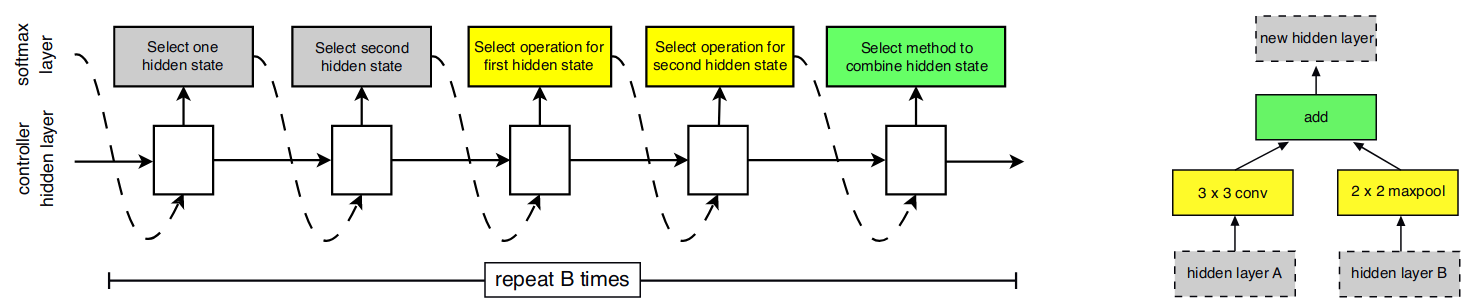
\includegraphics[width=\textwidth]{images/RL_conv_cell}
	%\pause
	%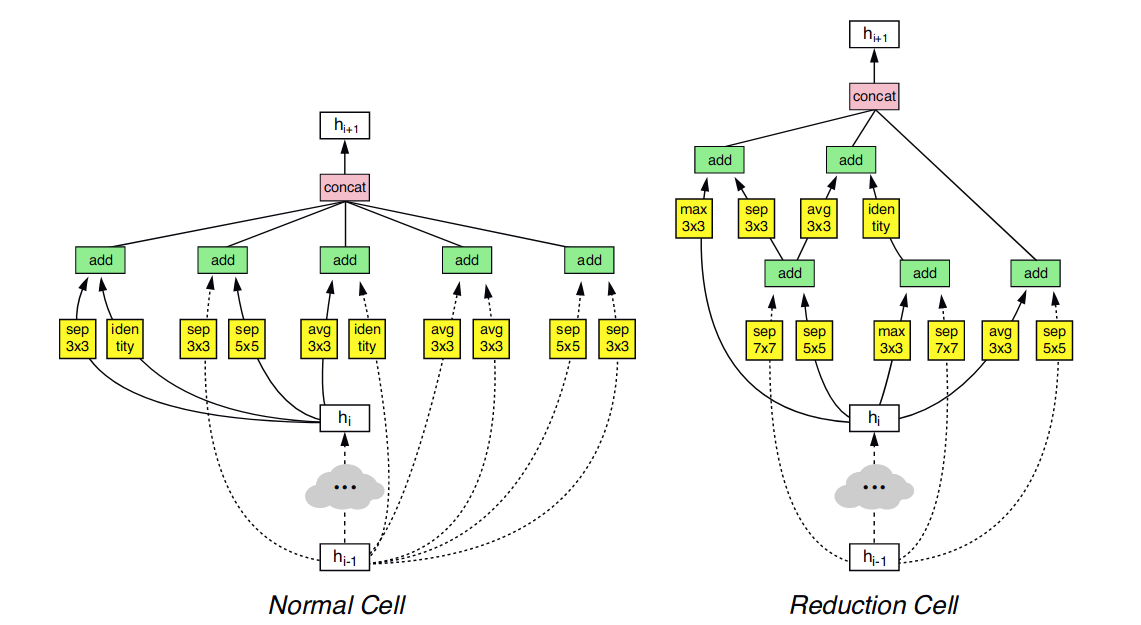
\includegraphics[width=.5\textwidth]{images/RL_normal_reduction}
	
}
%----------------------------------------------------------------------

%----------------------------------------------------------------------
\myframetop{Example of an architecture sample with B=5}{
\centering
\begin{columns}
	\column{0.3\textwidth}
	\centering
	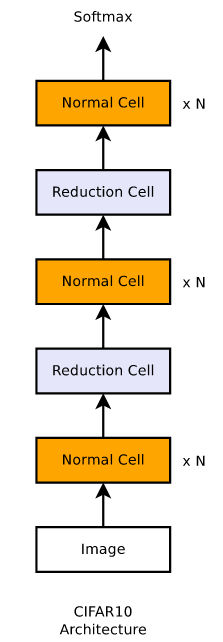
\includegraphics[width=.5\textwidth]{images/nasnet_full_net.png}

%\vspace{5cm}	
	\column{0.68\textwidth}
	\centering
	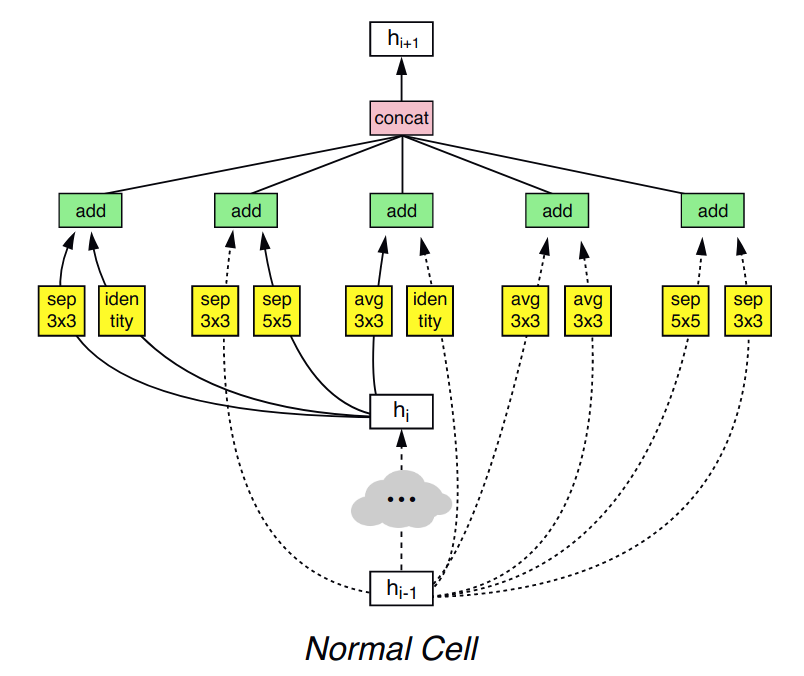
\includegraphics[width=.47\textwidth]{images/nasnet_normal.png}
	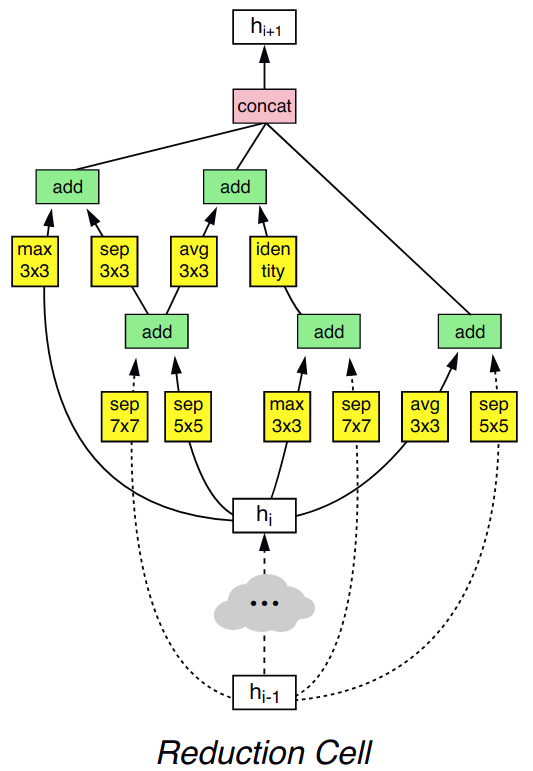
\includegraphics[width=.35\textwidth]{images/nasnet_reduce.png}
\end{columns}

\centering
Source: \lit{\href{https://openaccess.thecvf.com/content_cvpr_2018/papers/Zoph_Learning_Transferable_Architectures_CVPR_2018_paper.pdf}{Zoph et al. 2018}}
}
%----------------------------------------------------------------------

%----------------------------------------------------------------------
\myframe{Pros and Cons of Cell Search Space}{
\centering
What are some pros and cons of the cell search space compared to the basic one?\\~\\
Please think about this for a few minutes before continuing.
}
%----------------------------------------------------------------------

%----------------------------------------------------------------------
\myframe{Pros and Cons of Cell Search Space}{
\centering
\alert{Pros:}
\begin{itemize}
	\item Reduced search space size; speed-ups in terms of search time.
	\item Transferability to other datasets (e.g., cells found on
	CIFAR-10 transfer to ImageNet)
	\item Stacking repeating patterns is proven to be a useful design principle 
	(ResNet, Inception, etc.)
\end{itemize}
\pause
\medskip
\alert{Cons:}
\begin{itemize}
	\item Still need to (manually) determine the \textit{macro} architecture, 
	i.e., the way in which cells are connected.
	\item Limiting if different cells work better in different parts of the network
	\myit{
		\item[-] E.g., different spatial resolutions may favour different convolutions
	}
%	, e.g., different cells would be best at the beginning and end of the network.
\end{itemize}

}
%----------------------------------------------------------------------

%----------------------------------------------------------------------
\myframe{Hierarchical representation of search space \litw{\href{https://openreview.net/pdf?id=BJQRKzbA-}{Liu et al. 2017}}}{
	\centering
	\myit{
		\item Directed Acyclic Graph (DAG) representation of architectures
		\myit{
			\item[-] Each node is a latent representation; each edge is an operation/motif
		}
	\medskip		
	\pause
		\item There are different \alert{levels} of motivs
		\myit{
%			\item E.g. $o_1^{(2)}$ is a level-2 motif, $o_1^{(3)}$ is a level-3 motif
			\item \alert{Level-1 primitives}: standard operators; e.g., 3x3 conv, max pooling, \ldots
	\medskip		
	\pause
			\item \alert{Level-2 motivs}: combinations of level-1 primitives
		} 
	\centering
	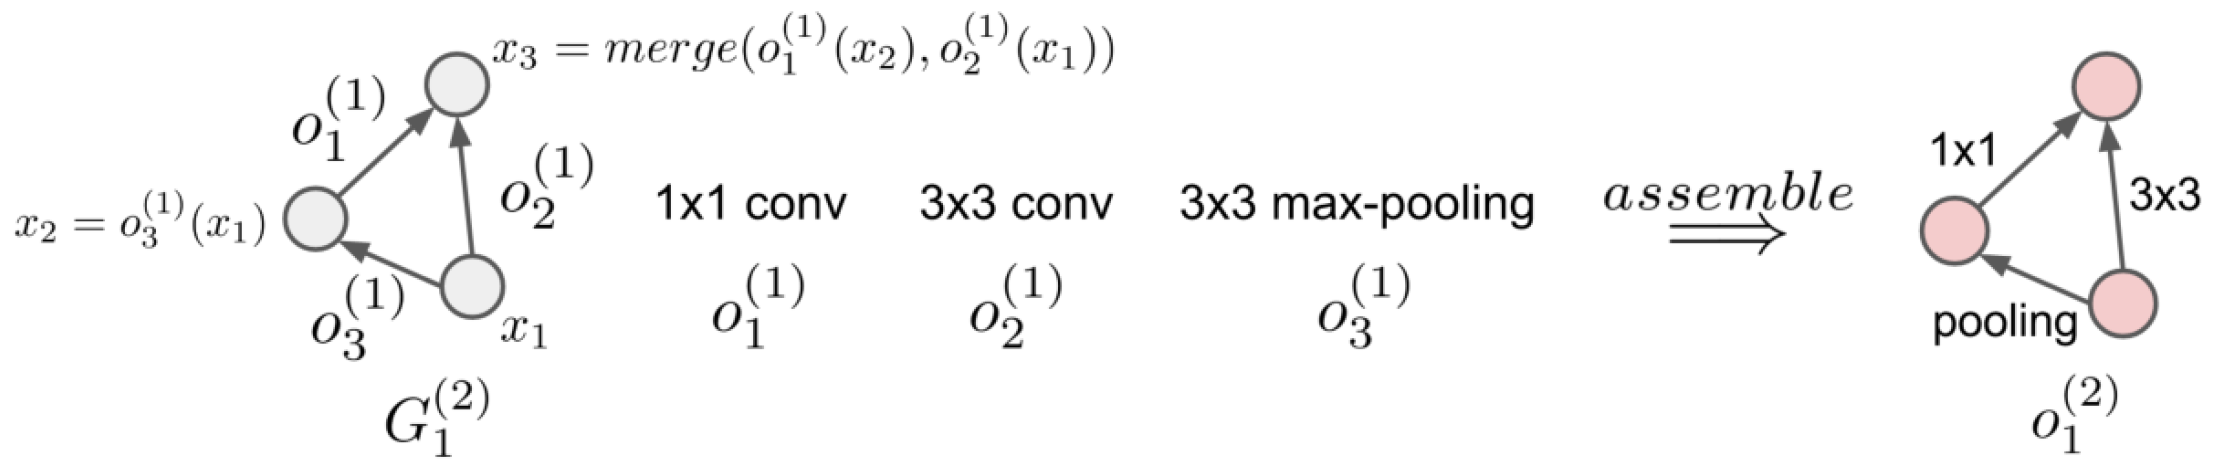
\includegraphics[width=0.6\textwidth]{images/hierarchical_nas_level1_2.png}
	\medskip		
	\pause
		\myit{
			\item \alert{Level-3 motivs}: combinations of level-2 motivs
		}
	\centering
	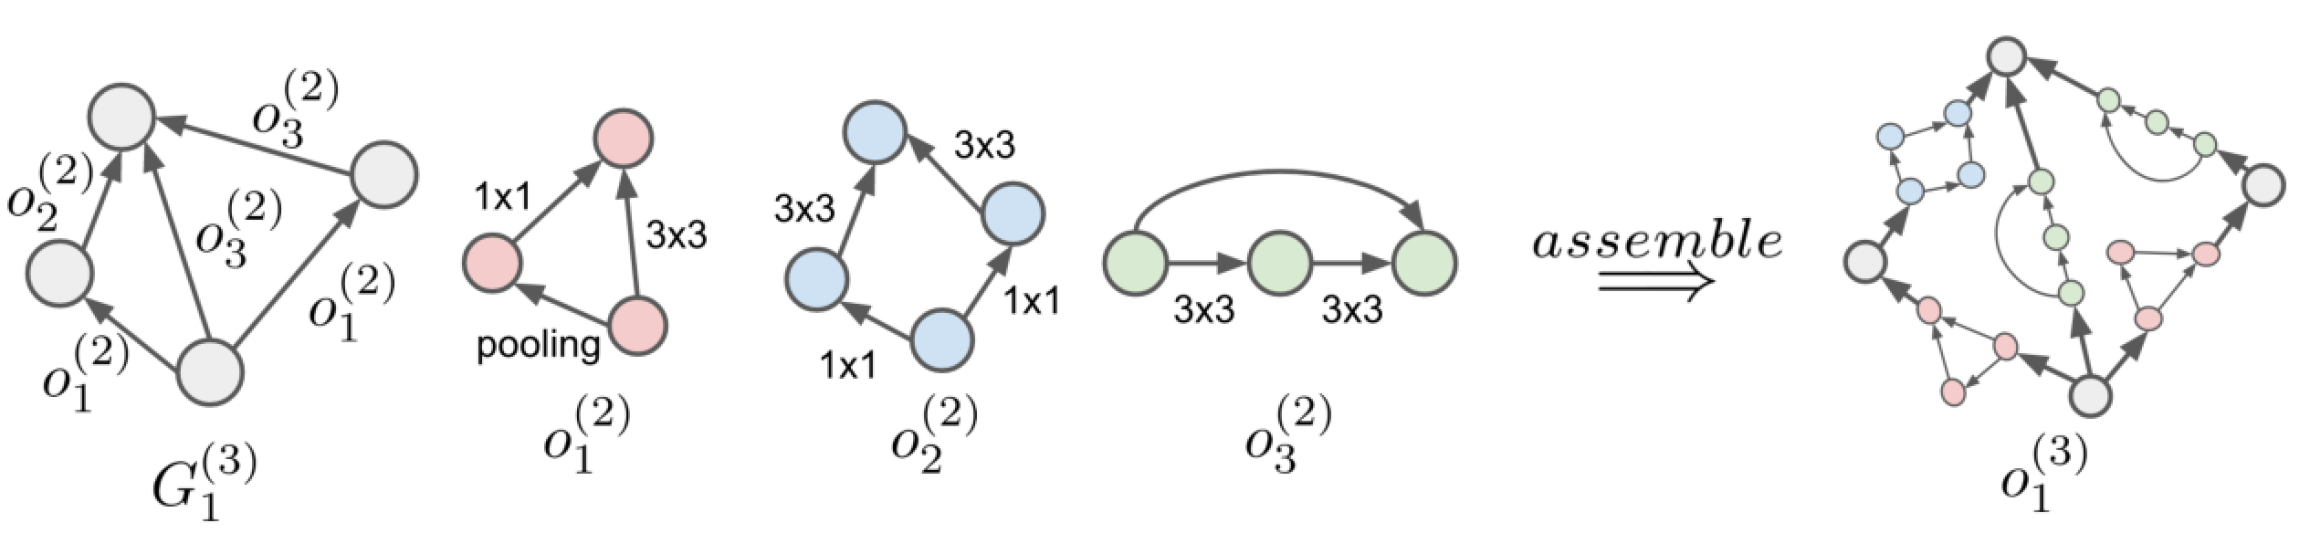
\includegraphics[width=0.6\textwidth]{images/hierarchical_nas_level2_3.png}
	}
%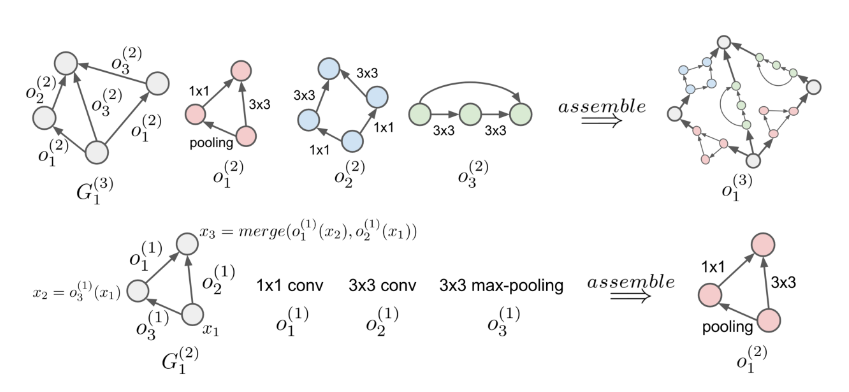
\includegraphics[width=\textwidth]{images/hierarchical_nas.png}\\
}
%----------------------------------------------------------------------

%----------------------------------------------------------------------
\myframe{Pros and Cons of Hierarchical Search Space}{
\centering
What are some pros and cons of a hierarchical search space compared to the cell search space?\\~\\
Please think about this for a few minutes before continuing.
}
%----------------------------------------------------------------------

%----------------------------------------------------------------------
\myframe{Pros and Cons of Hierarchical Search Space}{
	\centering
	\alert{Pros:}
	\begin{itemize}
		\item \alert{Flexibility} of \alert{constructing building blocks and reusing them many times}
		\myit{
			\item like a cell search space
		}
		\item \alert{Flexibility} of using different building blocks in different parts of the network
		\myit{
			\item like a basic search space
		}
		\item Ability to \alert{reuse building blocks at various levels of abstraction}
		\myit{
			\item again, this pattern has been used in manual design, e.g., in Inception nets
		}
	\end{itemize}
	\pause
	\bigskip
	\alert{Cons:}
	\begin{itemize}
		\item \alert{Larger} than cell search space
		\item Vastly more expressive than cell search space $\rightarrow$ \alert{potentially much harder to search}
	\end{itemize}
}
%----------------------------------------------------------------------


%----------------------------------------------------------------------
\myframe{Questions to Answer for Yourself / Discuss with Friends}{

	\myit{
		\item Repetition:\\ \alert{What are some pros and cons of the cell search space compared to the basic one?}
\bigskip
		\item Repetition:\\ \alert{Explain the way in which level-3 motivs in the hierarchical search space use level-2 motivs.}
\medskip
		\item Repetition:\\ \alert{What are some pros and cons of the hierarchical search space compared to the other ones?}
	}	 
}
%-----------------------------------------------------------------------



\videotitle{Blackbox Optimization Methods}

%-------------------------------------------------
%-------------------------------------------------
\myframe{Reinforcement Learning \litw{\href{https://arxiv.org/abs/1611.01578}{Zoph \& Le, 2017}}}{

{\begin{center}
	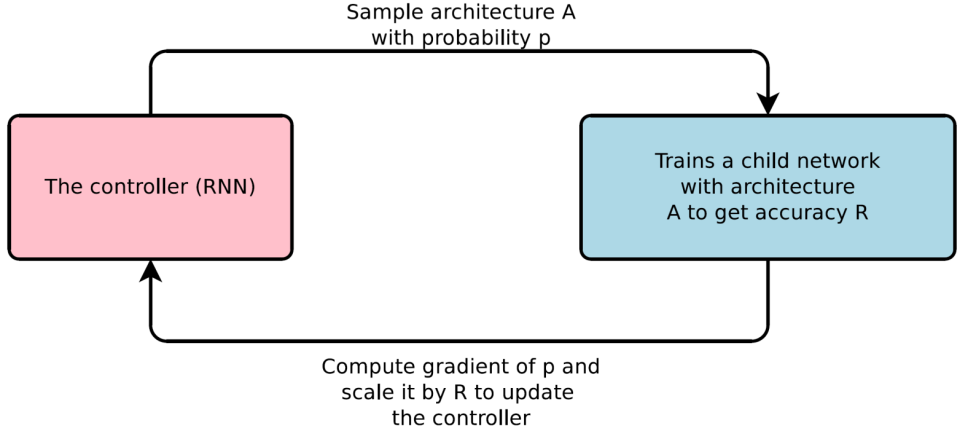
\includegraphics[width=.7\textwidth]{images/s27}
 \end{center}
}
\medskip
\begin{itemize}
	\item Use RNN ("\alert{Controller}") to generate a NN architecture piece-by-piece
	\item Train this NN ("\alert{Child Network}") and evaluate it on a validation set
	\item Use \alert{Reinforcement Learning (RL)} to update the parameters of the Controller 
	RNN to optimize the performance of the child models
\end{itemize}

}
%----------------------------------------------------------------------

%----------------------------------------------------------------------
\myframe{Learning CNNs with RL \litw{\href{https://arxiv.org/abs/1611.01578}{Zoph \& Le, 2017}}}{

\centering
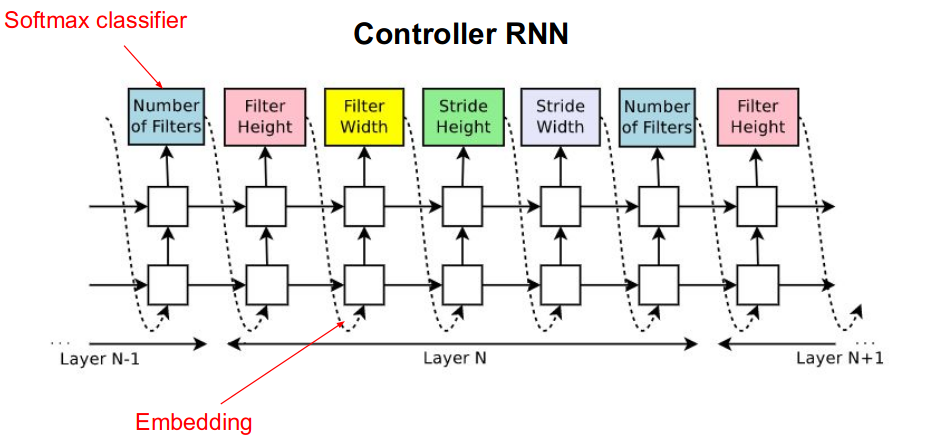
\includegraphics[width=.65\textwidth]{images/RL_CNN_controller}

\footnotesize{
	\myit{
	%	\item Maximize expected reward (validation accuracy): 
	%	$J(\theta_c)=E_{P(a_{1:T; \theta_c})}[R]$
		\item For a fixed number of layers, select:
		\begin{itemize}
			\item[-] \footnotesize Filter width/height, stride width/height, number of filters	
		\end{itemize}
	
	\pause
	\smallskip
		\item Large computational demands \alert{(800 GPUs for 2 weeks, 12.800 architectures evaluated)}
		%\myit{
		%	\item[-] \alert{800 GPUs for 2 weeks, 12.800 architectures evaluated}
		%}

	\pause
	\smallskip
	%	\item Each child model was trained for 50 epochs
	%	\item The final chosen architecture is trained for longer (600 epochs)
		%, optimizing the weights with SGD
		\item \alert{State-of-the-art results for CIFAR-10 \& Penn Treebank architecture}
		\myit{
			\item[$\rightarrow$] \footnotesize Brought NAS into the limelight
		}
	}
	}
}
%----------------------------------------------------------------------

%----------------------------------------------------------------------

\myframetop{Learning CNN cells with RL \litw{\href{http://openaccess.thecvf.com/content_cvpr_2018/html/Zoph_Learning_Transferable_Architectures_CVPR_2018_paper.html}{Zoph et al. ’18}}}{
	\centering
	
	\begin{itemize}
		\item 2 types of cells: normal and reduction cells
		\item For each type of cell: $B$ blocks, each with 5 choices
		\myit{
			\item[-] Choose two previous feature maps (from this cell)
			\item[-] For each of these, choose an operation (3$\times$3 conv, max-pool, etc.)
			\item[-] Choose a merge operation to combine the two results (concat or add)
		}
	
	\end{itemize}
	\bigskip
	\bigskip
	\smallskip
	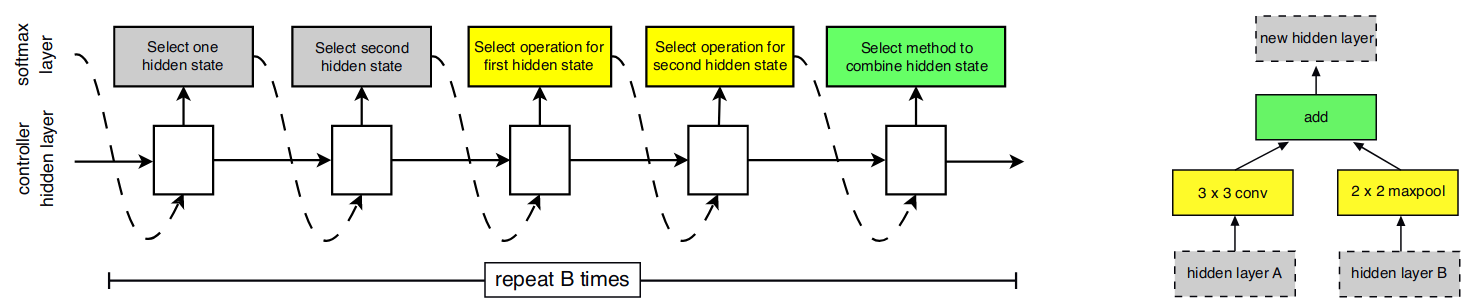
\includegraphics[width=\textwidth]{images/RL_conv_cell}
	%\pause
	%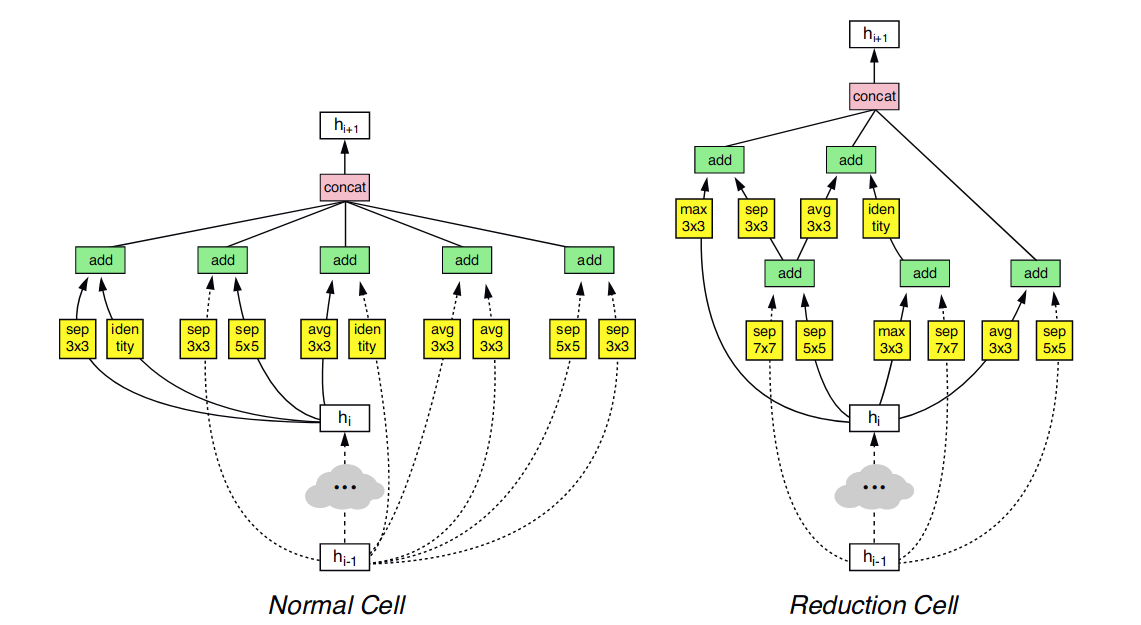
\includegraphics[width=.5\textwidth]{images/RL_normal_reduction}
	
}
%----------------------------------------------------------------------
%----------------------------------------------------------------------

\myframetop{NAS as Hyperparameter Optimization}{
	\begin{itemize}
		\item 2 types of cells: normal and reduction cells
		\item For each type of cell: $B$ blocks, each with 5 choices
		\myit{
			\item[-] Choose two previous feature maps (from this cell)
			\item[-] For each of these, choose an operation (3$\times$3 conv, max-pool, etc.)
			\item[-] Choose a merge operation to combine the two results (concat or add)
		}
	
	\end{itemize}
	\bigskip
	
	\begin{itemize}
	  \item This can be modelled as a HPO problem with 2$\times$5$\times$B variables:
	\end{itemize}
	~~~~~~\hspace*{0.08cm}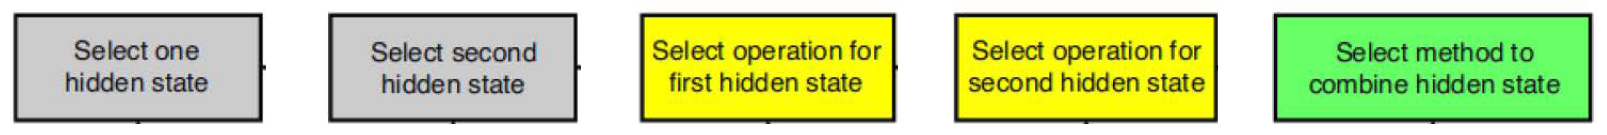
\includegraphics[width=0.613\textwidth]{images/NAS-RL-space_as_HPO}
	
}

%----------------------------------------------------------------------
%----------------------------------------------------------------------

\myframe{Evolution}{

\centering
\begin{enumerate}
	\footnotesize
	\item Initialize a \alert{population} of randomly sampled architectures.
	\item Sample pairs and select the architecture to mutate based on the \emph{fitness} function (e.g. validation error). \alert{Remove} the other from the population.
	\item Apply \alert{mutation} steps to the selected architecture, such as adding, changing or removing a layer. Add the new child architecture to the population. \lit{\href{https://arxiv.org/abs/1703.01041}{Real et al. 2017}; \href{https://openreview.net/forum?id=BJQRKzbA-}{Liu et al. 2017}; \href{https://arxiv.org/pdf/1703.00548.pdf}{Miikkulainen et al. 2017}}
\end{enumerate}

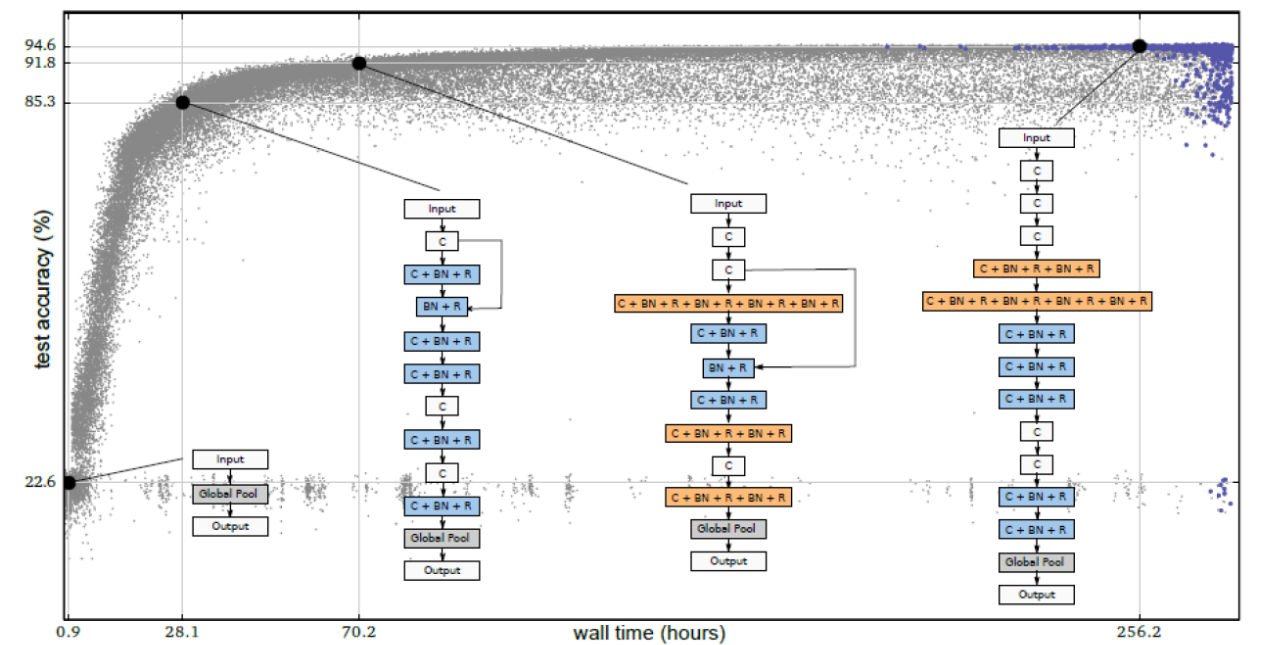
\includegraphics[width=.7\textwidth]{images/neuroevolution.png}\\

}
%----------------------------------------------------------------------

%----------------------------------------------------------------------
\myframe{Regularized/Aging Evolution \litw{\href{https://arxiv.org/abs/1802.01548}{Real et al, 2019}}}{

\centering
\begin{itemize}
	\footnotesize
	\item Standard evolutionary algorithm, but oldest solutions are dropped from
	population, instead of the worst.
	\item \alert{Evolution only for architectures; standard SGD for training weights}
	\item \alert{Same fixed-length (HPO) search space} as used for RL \lit{\href{http://openaccess.thecvf.com/content_cvpr_2018/html/Zoph_Learning_Transferable_Architectures_CVPR_2018_paper.html}{Zoph et al. ’18}}
\end{itemize}

\bigskip
\begin{columns}[T]

\column{0.4\textwidth}
\onslide<2->{
\centering
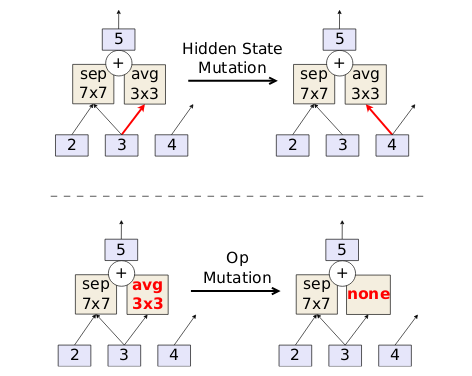
\includegraphics[width=\textwidth]{images/aging_evolution_mutations.png}
\footnotesize{Different types of mutations in cell search space}
}
\column{0.4\textwidth}
\onslide<3->{
\centering
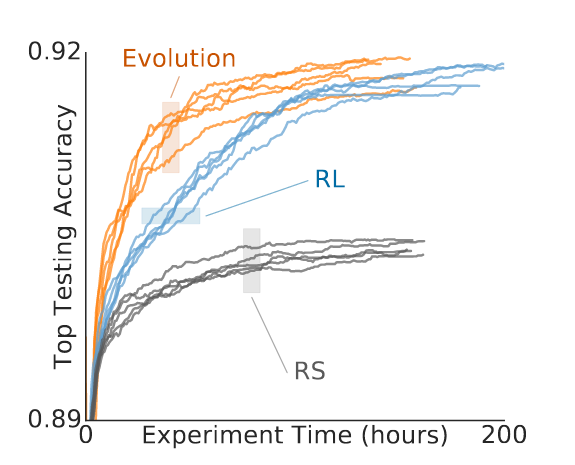
\includegraphics[width=.9\textwidth]{images/aging_evolution_results.png}
\footnotesize{State-of-the-art performance in apples-to-apples comparison\\ $\rightarrow$ \alert{AmoebaNet}}
}
\end{columns}

}
%----------------------------------------------------------------------

%----------------------------------------------------------------------
\myframe{Bayesian Optimization (BO)}{
	\myit{
		\item Encode the architecture as a vector space (like regularized evolution)
		\lit{\href{http://proceedings.mlr.press/v28/bergstra13.pdf}{Bergstra et al. 2013}, \href{https://ml.informatik.uni-freiburg.de/papers/15-IJCAI-Extrapolation_of_Learning_Curves.pdf}{Domhan et al. 2015}, \href{https://ml.informatik.uni-freiburg.de/papers/16-AUTOML-AutoNet.pdf}{Mendoza et al. 2015}, \href{https://arxiv.org/abs/1807.06906}{Zela et al. 2018}}
\pause
\medskip
		\item Joint optimization of architecture and hyperparameters, already in Auto-Net \lit{\href{https://ml.informatik.uni-freiburg.de/papers/16-AUTOML-AutoNet.pdf}{Mendoza et al. 2016}}
		\myit{
			\item[-] Based on BO with a random forest model (SMAC \lit{\href{https://ml.informatik.uni-freiburg.de/papers/11-LION5-SMAC.pdf}{Hutter et al, 2011}}) 
			\item[-] \alert{First automated deep learning (Auto-DL) method to win a machine learning competition dataset against human experts}
		}
\pause
\medskip
		\item Kernels for GP-based NAS
		\myit{
			\item[-] Arc kernel \lit{\href{https://ml.informatik.uni-freiburg.de/papers/13-BayesOpt_Arc-Kernel.pdf}{Swersky et al, 2013}}
			\item[-] NASBOT \lit{\href{https://arxiv.org/abs/1802.07191}{Kandasamy et al, 2018}}
		}
\pause
\medskip		
		\item There are also several recent promising BO approaches based on neural networks
		\myit{
			\item[-] BANANAS \lit{\href{https://arxiv.org/abs/1910.11858}{White et al. 2020}}
		}
		\item BO is very competitive, has been shown to outperform RL \lit{\href{http://proceedings.mlr.press/v97/ying19a.html}{Ying et al, 2019}}
	}
}
%-----------------------------------------------------------------------

%----------------------------------------------------------------------
%\myframe{Case study: NASBOT \litw{\href{https://arxiv.org/abs/1802.07191}{Kandasamy et al., NeurIPS 2018}}}{
%
%\centering
%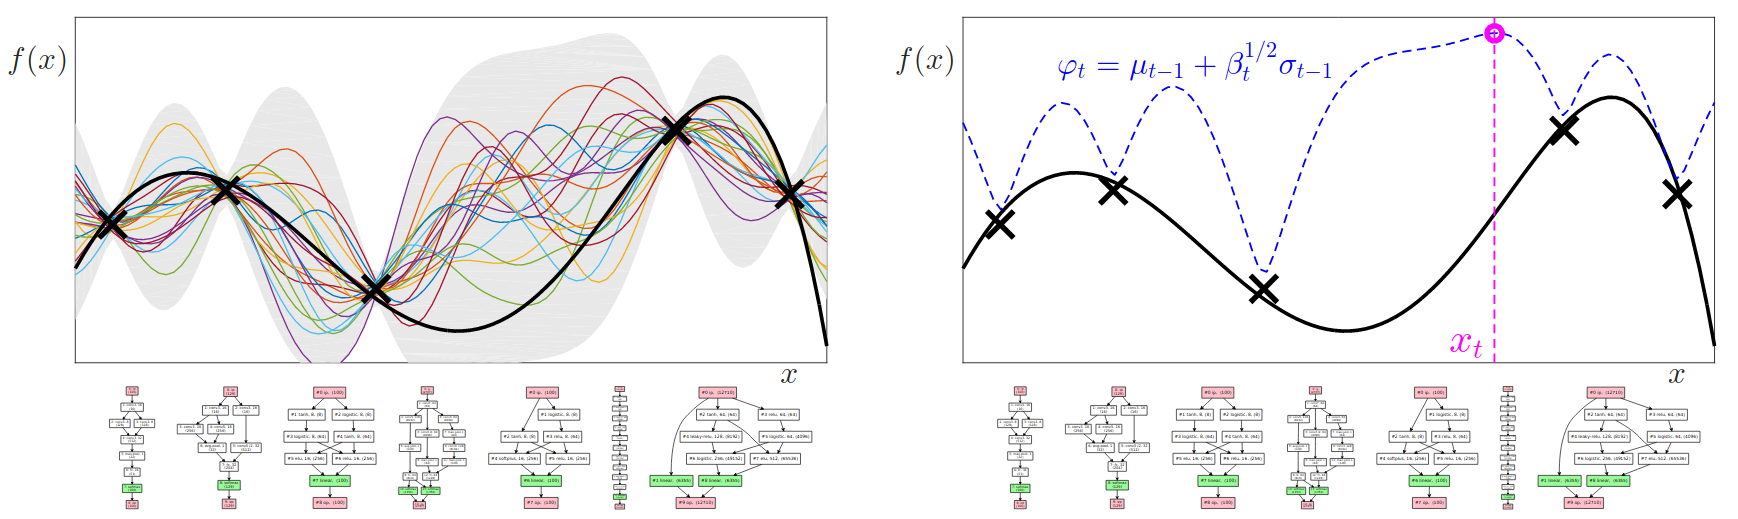
\includegraphics[width=.9\textwidth]{images/nasbot_1.png}
%\myit{
%\footnotesize
%		\item Gaussian Process BO is not that straighforward in non-Euclidian spaces such as the space of neural architectures
%		\myit{
%		\footnotesize
%			\item How to define a kernel (which entails the distance) in the architecture space?
%			\item How to optimize the acquisition function?
%		}
%\pause
%\medskip
%		\item \alert{NASBOT}
%		\myit{
%		\footnotesize
%			\item defines a distance metric based on Optimal Transport (\alert{OTMANN})
%			\item optimizes the acquisition function using \alert{evolution}
%		}		
%}
%
%}
%
%%----------------------------------------------------------------------
%\myframe{Case study: NASBOT \litw{\href{https://arxiv.org/abs/1802.07191}{Kandasamy et al., NeurIPS 2018}}}{
%
%\centering
%
%\begin{columns}
%\column{.6\textwidth}
%\vspace{-7cm}
%\myit{
%		\item The kernel: $\kappa = e^{-\beta d^{p}}$, where $d$ is the OTMANN distance
%		\myit{
%			\item[--] To compute $d$ between two architectures $G_1$, $G_2$: match computation (layer mass) in layers in $G_1$ to $G_2$
%		}
%}
%\pause
%\medskip
%
%\myit{
%	\item $Z \in \mathtt{R}^{n_1 \times n_2}$
%	\myit{
%		\item $Z_{ij} \longleftarrow$ \alert{amount of matched mass} between layer $i\in G_1$ and $j \in G_2$
%	}
%	\medskip
%	\item $d \triangleq \argminA_Z \phi_{lmm}(Z) + \phi_{str}(Z) + \phi_{nas}(Z)$
%	\myit{
%		\item[--] $\phi_{lmm}(Z)$: label mismatch penalty
%		\item[--] $\phi_{str}(Z)$: structural penalty
%		\item[--] $\phi_{nas}(Z)$: non-assignment penalty
%	}
%}
%
%\column{.4\textwidth}
%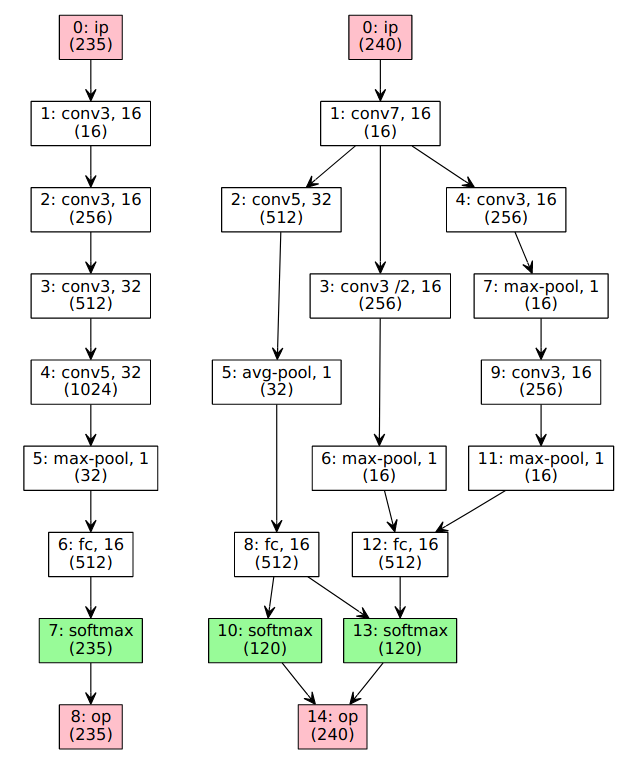
\includegraphics[width=\textwidth]{images/nasbot_2.png}
%
%\end{columns}
%
%}
%%-----------------------------------------------------------------------

%----------------------------------------------------------------------
\myframe{Questions to Answer for Yourself / Discuss with Friends}{

	\myit{
		\item Repetition:\\ 
		\alert{What are some pros and cons of using black-box optimizers for NAS?}
\medskip
		\item Repetition:\\
		\alert{How can NAS be modelled as a HPO problem?}
		%\item Repetition: \alert{Which blackbox NAS approach popularized the field?}
%\medskip
%		\item Repetition: \alert{Which blackbox NAS approach works best (to date)?}
\medskip
		\item Discussion:\\ \alert{Given enough resources, will blackbox NAS approaches always improve performance?}
\medskip
		\item Discussion:\\ \alert{Why does discarding the oldest individual (rather than the worst) help in Regularized/Aging evolution?}
	}	 
}
%-----------------------------------------------------------------------


\renewcommand{\lecturetitle}{NAS-Bench-101: The first NAS benchmark}
\renewcommand{\lecturetime}{Week 9, Video 4}
\section{\lecturetitle}
%-------------------------------------------------
%-------------------------------------------------

%----------------------------------------------------------------------
\myframe{Reproducibility crisis in NAS and the necessity of NAS benchmarks}{

\myit{
	\item \textit{\color{red}{Problem:}} Most of the NAS methods we saw so far are \alert{extremely difficult to reproduce and compare} (see \lit{\href{https://arxiv.org/pdf/1902.07638.pdf}{Li \& Talwalkar, 2019}; \href{https://arxiv.org/pdf/1909.02453.pdf}{Lindauer \& Hutter, 2020}}) due to:
	\myit{
		\item[--] Different search spaces
		\item[--] Different training pipelines
		\item[--] Other confounding factors such as different hardwares, different deep learning library versions, etc.
		\item[--] Industry-scale computational resources are not accessible to everyone	
		\item[--] No publicly available code
	}
\pause
\medskip
	\item \textit{\color{red}{Solution:}} A benchmark for NAS methods
}


\begin{center}
\begin{minipage}{0.8\textwidth}
\begin{block}{Definition: NAS Benchmark \litw{\href{https://arxiv.org/pdf/1909.02453.pdf}{Lindauer \& Hutter, 2020}}}
\textit{A NAS benchmark consists of a dataset (with a predifiend training-test split), a search space, and available runnable code with pre-defined hyperparameters for training the architectures.}
\end{block}
\end{minipage}
\end{center}

}
%-----------------------------------------------------------------------

%----------------------------------------------------------------------
\myframe{NAS-Bench-101: The first NAS benchmark \litw{\href{http://proceedings.mlr.press/v97/ying19a.html}{Ying et al, 2018}}}{

\centering
\myit{
	\item Cell-structured search space consisting of all directed acyclic graphs (DAGs) \\ on $V$ nodes, where each possible node has $L$ operation choices.
	\pause
	\item To limit the number of architectures, NAS-Bench-101 has the following constraints:
	\myit{
		\item $L = 3$ operators:
			\begin{columns}
			\column{.18\textwidth}
			- $3 \times 3$ convolution
			\column{.18\textwidth}
			- $1 \times 1$ convolution
			\column{.2\textwidth}
			- $3 \times 3$ max-pooling			
			\end{columns}
		\item $V \leq 7$ nodes
		\item A maximum of 9 edges
	}
}

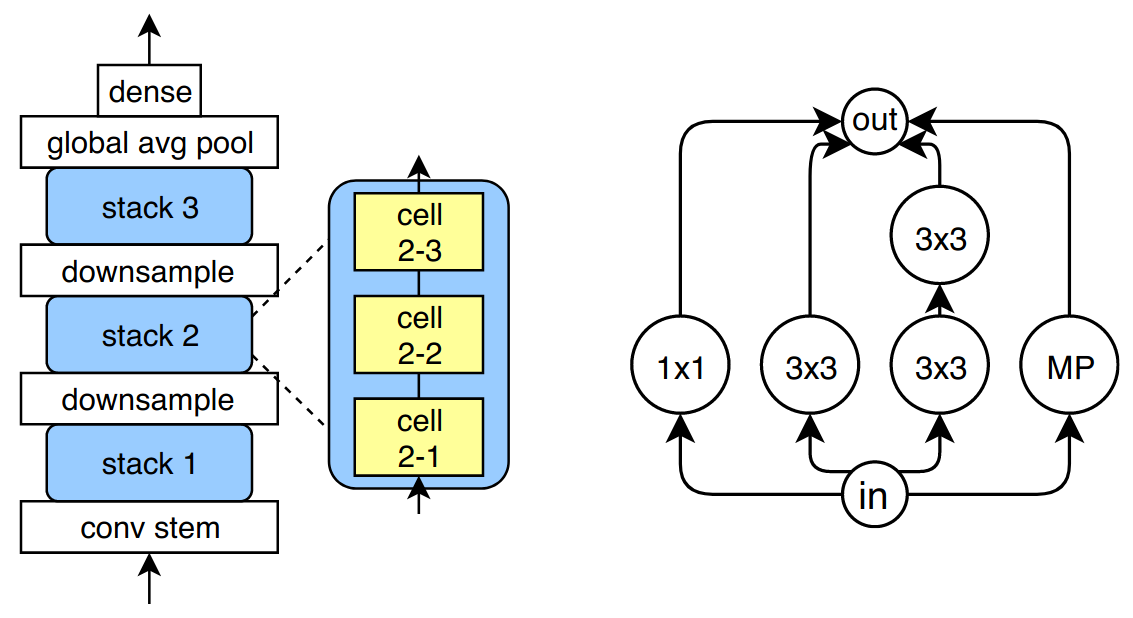
\includegraphics[width=.5\textwidth]{images/nasbench101_graph.png}

}
%-----------------------------------------------------------------------

%----------------------------------------------------------------------
\myframe{NAS-Bench-101: The first NAS benchmark \litw{\href{http://proceedings.mlr.press/v97/ying19a.html}{Ying et al, 2018}}}{

\centering
\myit{
	\item \alert{Tabular benchmark}: we exhaustively trained and evaluated all possible models on CIFAR-10 to create a tabular (look-up table) benchmark
	\item Based on this table, anyone can now run NAS experiments in seconds without a GPU.
}

\begin{columns}
\column{.6\textwidth}
\vspace{-2.7cm}
\myit{
	\onslide<2->{
		\item Around 423k \alert{unique} cells
		\myit{
			\item[--] 4 epoch budgets: 4, 12, 36, 108
			\item[--] 3 repeats
			\item[--] around 5M trained and evaluated models
			\item[--] 120 TPU years of computation
			\item[--] the best architecture mean test accuracy: 94.32\%
			}
	}
	\medskip
	\onslide<3->{
		\item Given an architecture encoding $A$, budget $E_{stop}$ and trial number, one can query from NAS-Bench-101 the following quantities:
		\myit{
			\item[--] training/validation/test accuracy
			\item[--] training time in seconds
			\item[--] number of trainable model parameters
		}
	}
}

\column{.375\textwidth}
\onslide<2->{
	%\vspace{-3cm}
	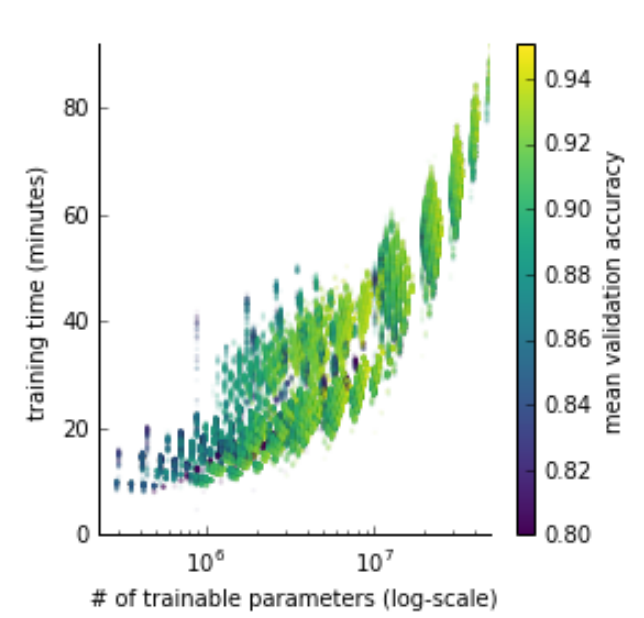
\includegraphics[width=.5\textwidth]{images/nasbench101_stat1.png}\\
	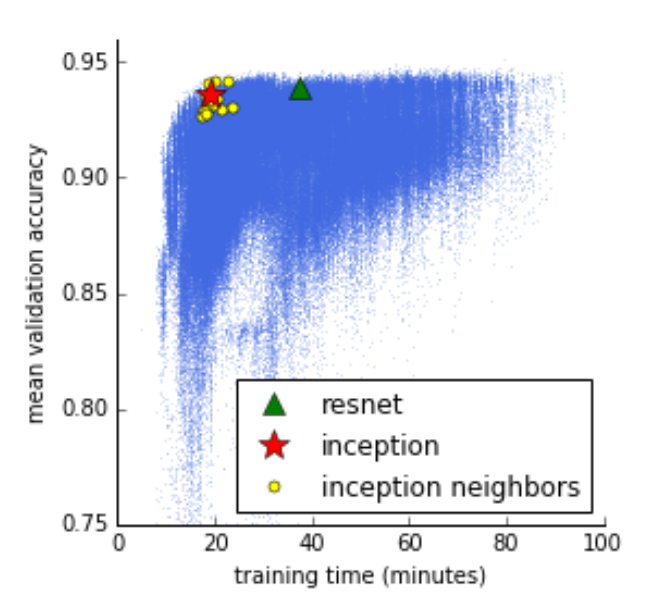
\includegraphics[width=.53\textwidth]{images/nasbench101_stat2.png}
}
\end{columns}

}
%-----------------------------------------------------------------------

%----------------------------------------------------------------------
\myframe{Blackbox NAS Methods on NAS-Bench-101 \litw{\href{http://proceedings.mlr.press/v97/ying19a.html}{Ying et al, 2018}}}{
	\myit{
%		\item All methods find good architectures
		\item RL outperforms random search
		\item BO and regularized evolution perform best, better than RL
	}
	\centering
	\medskip
	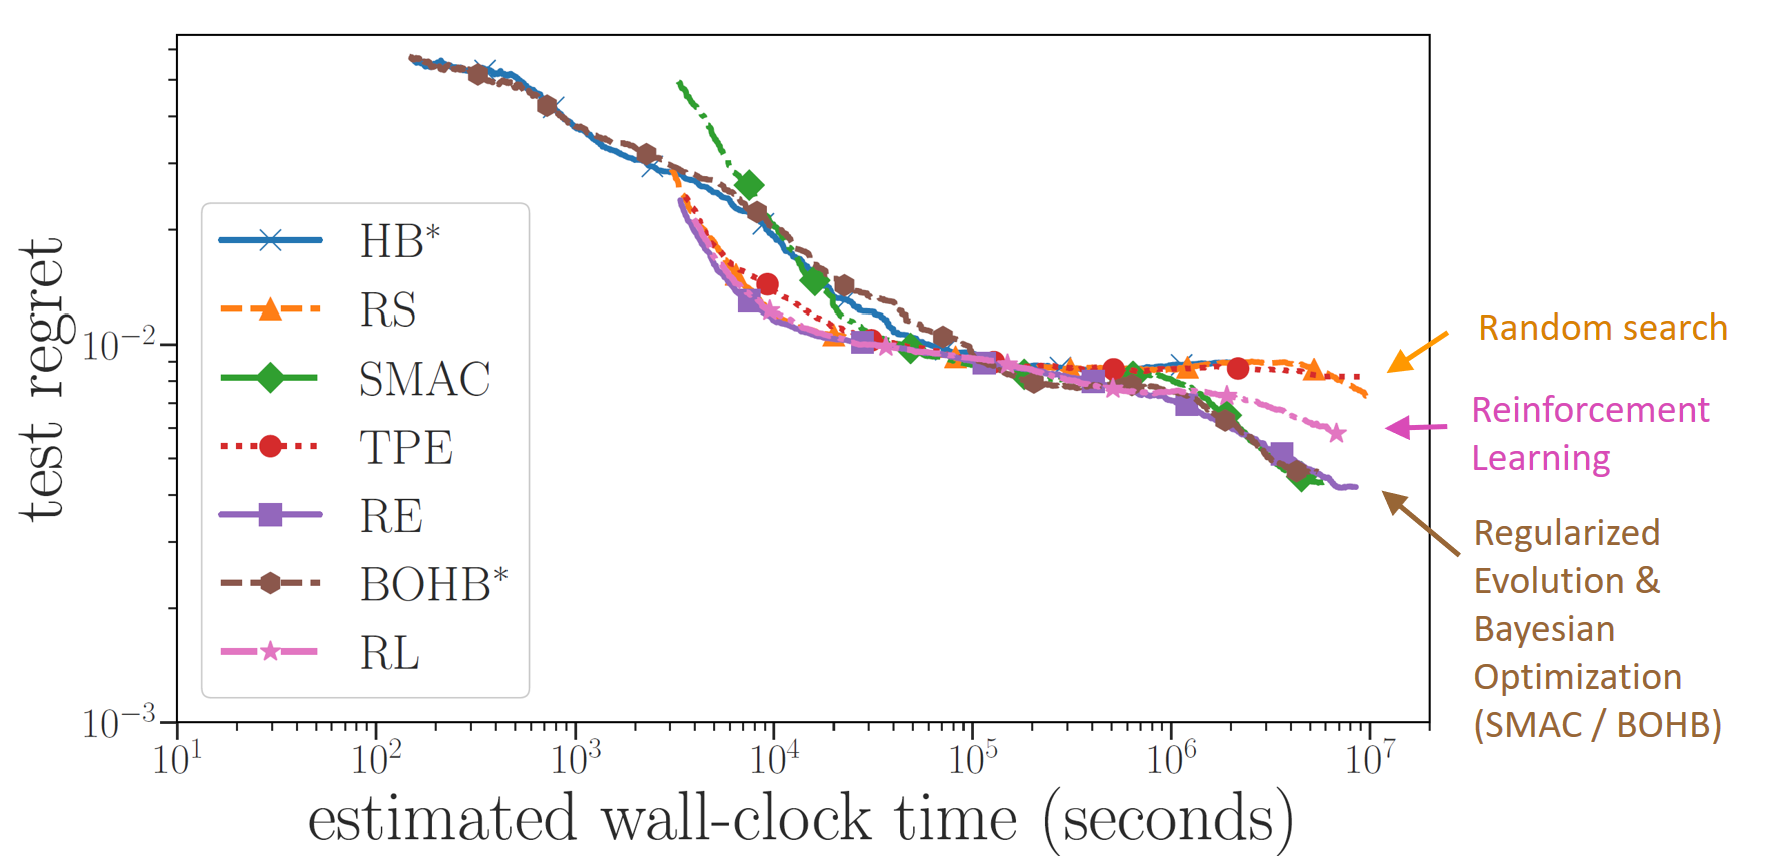
\includegraphics[width=0.65\textwidth]{images/NAS-Bench-101-results-with-labels}

\pause
	\myit{
		\item Note that the BO method SMAC \lit{\href{https://link.springer.com/chapter/10.1007/978-3-642-25566-3_40}{Hutter et al, 2011}} predated RL for \\NAS \lit{Zoph \& Le, 2017} by 6 years
		\myit{
			\item[-] Only now, benchmarks like NAS-Bench-101 allow for efficient comparisons
		}
	}
}
%-----------------------------------------------------------------------

%----------------------------------------------------------------------
\myframe{Questions to Answer for Yourself / Discuss with Friends}{

	\myit{
		\item Repetition:\\ 
		\alert{Why do we need proper benchmarking of NAS algorithms?}
		\item Repetition:\\
		\alert{What does a NAS benchmark subsume?}
	}	 
}
%-----------------------------------------------------------------------
\renewcommand{\lecturetitle}{Multi-fidelity approaches}
\renewcommand{\lecturetime}{Week 9, Video 5}
\section{\lecturetitle}
%-------------------------------------------------
%-------------------------------------------------


\renewcommand{\lecturetitle}{Network morphisms and weight inheritance}
\renewcommand{\lecturetime}{Week 9, Video 6}
\section{\lecturetitle}
%-------------------------------------------------
%-------------------------------------------------



\end{document}
